% FILE: sentiment_lexica.tex  Version 0.01
% AUTHOR: Uladzimir Sidarenka

% This is a modified version of the file main.tex developed by the
% University Duisburg-Essen, Duisburg, AG Prof. Dr. Günter Törner
% Verena Gondek, Andy Braune, Henning Kerstan Fachbereich Mathematik
% Lotharstr. 65., 47057 Duisburg entstanden im Rahmen des
% DFG-Projektes DissOnlineTutor in Zusammenarbeit mit der
% Humboldt-Universitaet zu Berlin AG Elektronisches Publizieren Joanna
% Rycko und der DNB - Deutsche Nationalbibliothek

\section{Sentiment Lexica}\label{sec:snt:lex}

The first avenue that we are going to explore with the help of the
obtained data set is an automatic prediction of polar terms.
% To this end, we will first present an updated version of our dataset
% in Subsection~\ref{subsec:snt-lex:data} in which our experts revised
% the annotations of words and idioms that were present in the existing
% German sentiment lexica (GSL), but were not marked as emo-expressions
% in our data and, vice versa, were annotated as polar terms in the
% corpus, but absent in the analyzed polarity lists.
For this purpose, we first evaluate the existing German sentiment
lexica on our corpus.  Since almost all of these resources were
created using an automatic translation of English polarity lists with
a manual post-editing of the translated entries, we then look whether
the original English sentiment lexicon generation (SLG) methods would
produce comparable results when applied to German data directly.
Finally, we analyze whether one of most popular areas of research in
contemporary computational linguistics---distributed vector
representations of words \cite{Mikolov:13}---could be a more
perspective way for deriving new domain-specific sentiment lexicons in
an unsupervised way.  In the concluding step, we investigate the
effects of different hyper-parameters and seed sets on these automatic
approaches, summarizing and concluding our experiments in the last
part of this section.

\subsection{Data}\label{subsec:snt-lex:data}

As we are interested in modelling a situation where no annotated
training data are available (thus looking for the most efficient
unsupervised SLG technique) but still want to evaluate the results in
a thorough way, we use the complete data set labeled by one of the
experts as our test corpus.  This set comprises a total of 6,040
positive and 3,055 negative terms.  However, since many of these
expressions are emoticons, which, on the one hand, are a priory absent
in common lexical taxonomies such as \texttt{WordNet}
\cite{Miller:95,Miller:07} or \texttt{GermaNet} \cite{Hamp:97} and
therefore not amenable to dictionary-based SLG approaches but, on the
other hand, can be easily captured by regular expressions, we decided
to exclude non-alphabetic smileys altogether from our study.  This
left us with a set of 3,459 positive and 2,755 negative labeled terms
(1,738 and 1,943 unique expressions respectively), whose
$\kappa$-agreement run up to 0.59.  In addition to that, we also
selected a small subset of 400 tweets from the other annotator and
used it as development data for tuning hyper-parameters of tested
approaches.

\subsection{Evaluation Metrics}\label{subsec:snt-lex:eval-metrics}

A central question to our subsequent experiments are the evaluation
metrics that we should use to measure the quality of (semi-)automatic
sentiment lexicons.  Usually, this quality is estimated either
\textit{intrinsically} (i.e., taking a lexicon in isolation and
immediately assessing its accuracy) or \textit{extrinsically} (i.e.,
considering the lexicon within the scope of a bigger application such
as a supervised classifier which utilizes lexicon's entries as
features).

Traditionally, intrinsic evaluation of English polarity lists amounted
to comparing these lists with the General Inquirer lexicon \cite[GI;
][]{Stone:66}---a manually compiled set of 11,895 words annotated with
their semantic categories---by taking the intersection of the two
resources and estimating the percentage of matches in which
automatically induced polar terms had the same polarity as the GI
entries.  This evaluation method, however, is somewhat problematic:
First of all, it is not easily transferable to other languages, since
even a manual translation of GI is not guaranteed to cover all
language-specific polar expressions.  Secondly, due to the
intersection, this method does not penalize for a low recall so that a
lexicon consisting of just two terms \textit{good}$^+$ and
\textit{bad}$^-$ will have the highest possible score, often
surpassing polarity lists with a greater number of entries.  Finally,
this comparison does not account for polysemy so that an ambiguous
word only one of whose (possibly rare) senses is subjective will
always be ranked the same as a purely polar term.

Unfortunately, an extrinsic evaluation does not always provide a
solution in this case, since, depending on the type of the extrinsic
system (e.g., a document classifier), it might still presuppose a
large data set for training other system components and, furthermore,
might yield overly high scores, which, however, are mainly due to
these extrinsic components rather than the quality of the lexicon
itself.

Instead of using these approaches, we opt for a direct comparison of
the induced lexicons with an annotated corpus, since this type of
evaluation allows us to solve at least three of the previously
mentioned issues: It does account for the recall, it does accommodate
polysemous words,\footnote{The annotators of the PotTS corpus were
  asked to annotate a polar expression iff its actual sense in the
  respective context was polar.} and it does preclude intermediate
modules which might artificially boost the results.  In particular, in
order to check a lexicon against the PotTS data set, we construct a
case-insensitive trie \cite[pp. 492--512]{Knuth:98} from the lexicon
entries and match this trie against the corpus text, simultaneously
comparing these entries with the actual word forms and lemmas of the
corpus tokens.\footnote{We use the \texttt{TreeTagger}
  \cite{Schmid:95} to obtain the lemma forms for the corpus tokens.} A
match is considered correct iff the matched lexicon entry absolutely
corresponds to the (possibly lemmatized) expert's annotation and has
the same polarity as the one specified by the human coder.  That way,
we estimate the precision, recall, and \F{}-score for each particular
polarity class (positive, negative, and neutral), considering all
words absent in the lexicon as neutral.

% \subsection{Data}\label{subsec:snt-lex:data}

% In the following experiments, we will use the updated version 0.1.0 of
% the sentiment dataset introduced in the previous section.  The main
% changes included in this version are:
% \begin{inparaenum}[\itshape a\upshape)]
%   \item the revision of the annotated emotional expressions, and
%   \item the addition of the boolean attributes \emph{subjective-fact}
%     and \emph{uncertain} to the annotation scheme of these elements.
% \end{inparaenum}

% To accomplish the fortmer objective, we compared the labelings of the
% opinionated terms in the first release of our corpus (version 0.0.1
% presented previously) with the entries from the existing German
% sentiment lexica: SentiWS \cite{Remus:10}, German Polarity Clues
% \cite{Waltinger:10}, and the Zurich Polarity List \cite{Clematide:10}.
% Similarly to the adjudication procedure used earlier, we automatically
% highlighted the differences between the corpus labels and the entries
% of these resources, letting our experts resolve the emerged conflicts.

% As it turned out, many of the contradicting cases stemmed from a
% different treatment of polar facts, such as ``Tod'' (\emph{death}),
% ``Anstieg'' (\emph{surge}), ``duften'' (\emph{to scent}) etc.: these
% entities were not labeled as emo-expressions in the full annotation of
% our dataset, but were still present as opinionated terms in the
% analyzed polarity lists.  Since these words represented a special
% class of polar clues due to their unequivocal objective nature, we
% decided to introduce a special feature called \emph{subjective-fact}
% into the attribute set of emotional expressions, explicitly asking our
% coders to annotate such terms with the emo-expression tag, but setting
% the value of the newly added attribute to \texttt{true}.

% The remaining differences were mainly due to polysemous words whose
% meaning in the corpus was not always subjective; errors in the lexica
% (GPC, for example, featured such auxiliary terms as ``sein'' (\emph{to
%   be}), ``wer'' (\emph{who}), or ``aus'' (\emph{from}) as opinionated
% entries); and, finally, numerous borderline cases which were difficult
% to resolve even in group discussions.  Examples of such challenging
% cases were words and idioms such as ``verbieten'' (\emph{to
%   prohibit}), ``verwechseln'' (\emph{to confuse}), ``Hauen und
% Stechen'' (\emph{hewing and stabbing}).  To address this issue, we
% again introduced an additional attribute, called \emph{uncertain},
% into the annotation scheme of emotional expressions and asked our
% experts to mark such borderline instances with this attribute.

% The statistics on the total number of the labeled elements and their
% agreement in the updated version are shown in
% Table~\ref{tbl:snt-lex:ucrp-agrmnt}:

% \begin{table*}[thb!]
%   \begin{center}
%     \bgroup \setlength\tabcolsep{0.7\tabcolsep} \scriptsize
%     \begin{tabular}{p{0.15\textwidth} % first columm
%         *{10}{>{\centering\arraybackslash}p{0.05\textwidth}}} % next ten columns
%       \toprule
%           \multirow{2}{0.2\textwidth}{\bfseries Element} &
%           \multicolumn{5}{c}{\bfseries Binary $\kappa$} & %
%           \multicolumn{5}{c}{\bfseries Proportional $\kappa$}\\
%           \cmidrule(r){2-6}\cmidrule(l){7-11}
%           & $M_1$ & $A_1$ & $M_2$ & $A_2$ & $\mathbf{\kappa}$ %
%           & $M_1$ & $A_1$ & $M_2$ & $A_2$ & $\mathbf{\kappa}$\\\midrule

%           EExpression &  &  &  & & \textbf{} & &  &  &  & \textbf{}\\
%           \bottomrule
%     \end{tabular}
%     \egroup
%   \end{center}
%   \captionof{table}{Inter-annotator agreement on the emotional
%     expression in the updated corpus.\\ {\small ($M1$ -- number of
%       tokens with matching labels in the first annotation, $A1$ --
%       total number of tokens labeled with that class in the first
%       annotation, $M2$ -- number of tokens with matching labels in the
%       second annotation, $A2$ -- total number of tokens labeled with
%       that class in the second annotation)}}
%   \label{tbl:snt-lex:ucrp-agrmnt}
% \end{table*}

\subsection{Evaluation of the Existing German Lexica}

In order to obtain an upper bound of the expected scores for an
automatic prediction of polar terms, we evaluated the existing German
sentiment lexica on the annotated data of our corpus.  The most
prominent of these resources are:
\begin{itemize}
\item the \textbf{German Polarity Clues} (GPC) by
  \citet{Waltinger:10}, which comprises 10,141 subjective entries
  automatically translated from the English sentiment lexica
  Subjectivity Clues \cite{Wilson:05} and SentiSpin \cite{Takamura:05}
  with a subsequent manual correction of these translations and
  several synonyms and negated terms added by the authors;

\item the \textbf{SentiWS} (SWS) lexicon introduced by
  \citet{Remus:10}, which includes 1,818 positively and 1,650
  negatively connotated terms, also providing their part-of-speech
  tags and inflections (resulting in a total of 32,734 word forms).
  Similarly to the GPC, the authors used an English sentiment
  resource---the General Inquirer list by \citet{Stone:66}---to
  bootstrap the entries for their lexicon, manually revising these
  automatic translations afterwards.  In addition to that,
  \citet{Remus:10} also expanded their polarity set with words and
  phrases frequently co-occurring with positive and negative seed
  lexemes using collocation information obtained from a corpus of
  10,200 customer reviews or extracted from the German Collocation
  Dictionary \cite{Quasthoff:10};

\item and, finally, the \textbf{Zurich Polarity List} developed by
  \citet{Clematide:10}, which comprises 8,000 subjective entries taken
  from GermaNet synsets \cite{Hamp:97}.  These synsets were manually
  annotated with their prior polarities by human experts.  Since the
  authors, however, found the number of polar adjectives obtained that
  way insufficient for running further classification experiments,
  they automatically enriched their lexicon with more attributive
  terms by analyzing conjoined collocations from a corpus using the
  method of \citet{Hatzivassi:97}.
\end{itemize}

In order to evaluate these resources on our dataset, we represented
each of the above lexicons as a trie \cite[pp. 492--512]{Knuth:98}
with the lexicon entries corresponding to paths in the resulting graph
and the polarity class(es) of these entries stored at the respective
terminal leaf nodes.  We then applied the standard match operation by
simultaneously checking the trie against contiguous runs of both
original and lemmatized corpus tokens.  All lemmatizations were done
using the \texttt{TreeTagger} \cite{Schmid:95}, and the match
operation was made case-insensitive.  Furthermore, since all analyzed
lexica only included plain textual terms, we also ignored smileys
during this comparison, solely concentrating on common lexical terms.

In this way, we estimated the precision, recall, and \F{}-score of the
positive, negative, and neutral polarity classes\footnote{We
  considered a term as neutral if it was not featured in the lexicon
  as either positive or negative entry.} of each lexicon by separately
computing these figures on each corpus file (99--109 tweets) and then
obtaining the mean and standard deviation of these scores over all
files in the dataset.  In addition to that, we also calculated the
macro- and micro-averaged results over all polarity classes.
Following the standard practice for computing these terms, we
estimated the macro-average as the mean of the \F{}-scores over all
three types (positive, negative, and neutral) and obtained the
micro-average by taking the harmonic mean of precision and recall
calculated over all true positives, false positives, and false
negatives found in the corpus.  The results of these computations are
shown in Table~\ref{snt-lex:tbl:gsl-res}.\footnote{For the sake of
  these experiments, we excluded the auxiliary words ``aus''
  (\emph{from}), ``der'' (\emph{the}), ``keine'' (\emph{no}),
  ``nicht'' (\emph{not}), ``sein'' (\emph{to be}), ``was''
  (\emph{what}), and ``wer'' (\emph{who}) with their inflection forms
  from the German Polarity Clues lexicon, since these entries
  significantly worsened the evaluation results.}

\begin{table}[h]
  \begin{center}
    \bgroup \setlength\tabcolsep{0.1\tabcolsep}\scriptsize
    \begin{tabular}{p{0.162\columnwidth} % first columm
        *{9}{>{\centering\arraybackslash}p{0.074\columnwidth}} % next nine columns
        *{2}{>{\centering\arraybackslash}p{0.068\columnwidth}}} % last two columns
      \toprule
          \multirow{2}*{\bfseries Lexicon} & %
          \multicolumn{3}{c}{\bfseries Positive Expressions} & %
          \multicolumn{3}{c}{\bfseries Negative Expressions} & %
          \multicolumn{3}{c}{\bfseries Neutral Terms} & %
          \multirow{2}{0.068\columnwidth}{\bfseries\centering Macro\newline \F{}} & %
          \multirow{2}{0.068\columnwidth}{\bfseries\centering Micro\newline \F{}}\\
          \cmidrule(lr){2-4}\cmidrule(lr){5-7}\cmidrule(lr){8-10}

          & Precision & Recall & \F{} & %
          Precision & Recall & \F{} & %
          Precision & Recall & \F{} & & \\\midrule
      %% \multicolumn{9}{|c|}{\cellcolor{cellcolor}Existing Lexica}\\\hline

      GPC & 24\stddev{7.9} & 46.4\stddev{11.2} & 31.1\stddev{8.2} & %
      22\stddev{8.1} & 41.6\stddev{10.6} & 28.1\stddev{8.3} & %
      98\stddev{0.5} & 94.3\stddev{1} & 96.1\stddev{0.5} & %
      51.8\stddev{4.7} & 92.3\stddev{0.9}\\

      SWS & 35.9\stddev{13.2} & 38.7\stddev{11.6} & 36\stddev{9.9} & %
      49\stddev{17.1} & 31.3\stddev{10.9} & \textbf{37.2}\stddev{11.6} & %
      97.5\stddev{0.5} & 97.8\stddev{1} & 97.7\stddev{0.5} & %
      \textbf{56.9}\stddev{6.2} & 95.4\stddev{0.9}\\

      ZPL & 36.4\stddev{12.3} & 21.3\stddev{7.2} & 26.3\stddev{8} & %
      41.1\stddev{15.6} & 23.3\stddev{8.7} & 29\stddev{10} & %
      97\stddev{0.6} & 98.7\stddev{0.3} & 97.8\stddev{0.3} & %
      51.1\stddev{4.4} & 95.7\stddev{0.6}\\

      GPC $\cap$ SWS $\cap$ ZPL & \textbf{54}\stddev{12.8} & %
      30.6\stddev{10.5} & \textbf{38.1}\stddev{10.1} & %

      \textbf{61.7}\stddev{17.8} & 21.6\stddev{9.1} & 31.2\stddev{11.3} & %
      97.1\stddev{0.6} & \textbf{99.3}\stddev{0.3} & \textbf{98.2}\stddev{0.3} & %
      55.8\stddev{5.4} & \textbf{96.4}\stddev{0.6}\\

      GPC $\cup$ SWS $\cup$ ZPL & 23.3\stddev{7.6} & \textbf{48.5}\stddev{11.2} & %
      30.9\stddev{8.2} & %

      22\stddev{8} & \textbf{46.1}\stddev{10.8} & 29.1\stddev{8.5} & %
      \textbf{98.1}\stddev{0.5} & 93.9\stddev{1} & 96\stddev{0.5} & %
      52\stddev{4.8} & 92\stddev{0.9}\\\bottomrule
    \end{tabular}
    \egroup
    \caption{Evaluation of the existing German sentiment lexica.\\
      {\small (GPC -- German Polarity Clues \cite{Waltinger:10}, SWS
        -- SentiWS \cite{Remus:10}, ZPL -- Zurich Polarity Lexicon
        \cite{Clematide:10})}}
    \label{snt-lex:tbl:gsl-res}
  \end{center}
\end{table}

As can be seen from the table, the intersection of all three lexica
attains the best results on both positive and neutral classes, also
yielding the best scores in terms of the micro-averaged $F$-measure.
One of the main reasons for this success is a relatively high
precision of this list for all but the neutral polarity class, where
it is outperformed by the union of the three resources.  Not
surpisingly, the union also shows the highest recall of positive and
negative terms among all compared polarity lists.

Regarding the figures attained by the individual lexica, the best
results here are achieved by the SentiWS resource \cite{Remus:10},
which not only shows the highest \F{}-score for the negative terms but
also achieves the best macro-averaged \F{}-result on all classes.

At the same time, we also can observe that the deviation of the scores
on different files is relatively high.  In order to see whether this
skewness of the distribution could significantly affect the net
statistics, we additionally recomputed all results on the whole corpus
at once.  The updated figures are shown in
Table~\ref{snt-lex:tbl:gsl-res-full}.

\begin{table}[h]
  \begin{center}
    \bgroup \setlength\tabcolsep{0.1\tabcolsep}\scriptsize
    \begin{tabular}{p{0.162\columnwidth} % first columm
        *{9}{>{\centering\arraybackslash}p{0.074\columnwidth}} % next nine columns
        *{2}{>{\centering\arraybackslash}p{0.068\columnwidth}}} % last two columns
      \toprule
          \multirow{2}*{\bfseries Lexicon} & %
          \multicolumn{3}{c}{\bfseries Positive Expressions} & %
          \multicolumn{3}{c}{\bfseries Negative Expressions} & %
          \multicolumn{3}{c}{\bfseries Neutral Terms} & %
          \multirow{2}{0.068\columnwidth}{\bfseries\centering Macro\newline \F{}} & %
          \multirow{2}{0.068\columnwidth}{\bfseries\centering Micro\newline \F{}}\\
          \cmidrule(lr){2-4}\cmidrule(lr){5-7}\cmidrule(lr){8-10}

          & Precision & Recall & \F{} & %
          Precision & Recall & \F{} & %
          Precision & Recall & \F{} & & \\\midrule
      %% \multicolumn{9}{|c|}{\cellcolor{cellcolor}Existing Lexica}\\\hline

      GPC & 23.83 & 46.8 & 31.58 & %
       22.37 & 41.58 & 29 & %
       98.01 & 94.27 & 96.1 & %
       52.26 & 91.32\\

      SWS & 34.36 & 39.23 & 36.63 & %
       49.56 & 31.45 & \textbf{38.48} & %
       97.5 & 97.84 & 97.67 & %
       \textbf{57.59} & 95.38\\

      ZPL & 36.4 & 21.22 & 26.81 & %
       41.57 & 23.14 & 29.73 & %
       96.96 & 98.73 & 97.84 & %
       51.46 & 95.67\\

      GPC $\cap$ SWS $\cap$ ZPL & \textbf{54.52} & 30.74 & \textbf{39.31} & %
       \textbf{62.92} & 21.68 & 32.25 & %
       97.13 & \textbf{99.25} & \textbf{98.18} & %
       56.58 & \textbf{96.39}\\

      GPC $\cup$ SWS $\cup$ ZPL & 23.11 & \textbf{48.86} & 31.38 & %
       22.42 & \textbf{46.05} & 30.16 & %
       \textbf{98.14} & 93.87 & 95.96 & %
       52.5 & 91.99\\\bottomrule
    \end{tabular}
    \egroup
    \caption{Evaluation of the existing German sentiment lexica on the
      complete corpus.\\ {\small (GPC -- German Polarity Clues
        \cite{Waltinger:10}, SWS -- SentiWS \cite{Remus:10}, ZPL --
        Zurich Polarity Lexicon \cite{Clematide:10})}}
    \label{snt-lex:tbl:gsl-res-full}
  \end{center}
\end{table}

As we can see from the scores, the relative placement of the
best-performing systems is the same as in the previous evaluation.
Moreover, the absolute results are only minimally higher (by typically
at most one percent) than the mean values computed in the previous
step.  Thus, even despite their high variance, the average figures
computed over single corpus files are still a reliable indicator of
the quality of the recognized opinionated terms.  For the sake of
brevity, we will therefore only present the former metric (the mean
and standard deviation of the scores estimated over individual files),
refraining from computing the statistics on the whole corpus in total.

\subsection{Evaluation of Dictionary-Based Approaches}

Since all of the presented works rely on a manual correction or
partial annotation of the lexicon entries, they clearly fall into the
category of semi-automatic approaches.  Unlike fully automated
methods, such systems typically yield more precise results, which,
however, come at the cost of tedious human efforts.  In order to see
to which extent these efforts really pay off in practice for the
lexicon generation (LG) task at hand, we additionally decided to
evaluate the most popular fully automatic LG approaches.

According to \citet[p. 79]{Liu:12}, most of such automated methods can
be divided into dictionary- and corpus-based ones.  The former
approaches try to derive polarity lists using monolingual thesauri or
lexical databases such as the Macquarie Dictionary \cite{Bernard:86}
or \textsc{WordNet} \cite{Miller:95}.  A clear advantage of these
systems is their relatively good precision as they operate on
carefully verified data enriched with hand-crafted meta information.
At the same time, this verification can become a drawback for the
recall in the domains where the language changes occur very rapidly,
and new terms are being coined in a flash.

The presumably first such approach was proposed by \citet{Hu:04}.  In
their work on sentiment classification and summarization of cutomer
reviews, the authors determined semantic orientation of adjectives
(which were supposed to be the most relevant part of speech for mining
people's opinions) by taking a set of seed terms with known polarities
and propagating these values to the synonyms of these words that were
found in \textsc{WordNet} \cite{Miller:95}.  A similar procedure was
applied to antonymous relations with the polarity orientation being
reversed during the propagation.  This expansion continued until no
more adjective could be reached via the synonymy-antonymy links.
Unfortunately, no intrinsic evaluation of the resulting lexicon was
performed in this work---the authors only report their results on
recognizing subjective sentences and classifying their polarity, where
they attain average \F-scores of 0.667 and 0.842 respectively.

Later on, this approach was refined by \citet{Blair-Goldensohn:08},
who obtained polarity labels for new words by multiplying a score
vector $v$ containing polarity scores of the known seed terms (-1 for
the negative expressions and 1 for the positive terms) with the
adjacency matrix $A$ constructed from the \textsc{WordNet} synsets.
In these experiments, the value of the adjacency cell $a_{ij}$ in the
matrix $A$ was set to $\lambda=0.2$ if there was a synonymy link
between the synsets $i$ and $j$ and to $-\lambda$ if these synsets
were antonymous to each other.  By performing this multiplication
multiple times and setting the $v$ vector to the result of the
previous iteration, the authors ensured that the polarity scores were
being propagated transitively through the network, decaying by a
constant factor ($\lambda$) with the increasing path length from the
original seeds.  This method again was evaluated only
extrinsically---the authors tested their complete sentiment
summarization system, which used the sentiment scores for individual
words as features for a maximum-entropy classifier.

With various modifications, the core idea of propagating the polarity
classes through the semantic graph was adopted in almost all of the
following dictionary-based works: \citet{Kim:04,Kim:06}, for instance,
used a similar method to determine the polarity of adjectives and
verbs given a small seed set of terms with known orientations.  In
particular, the likelihood of a new word $w$ belonging to the class $c
\in \{\textrm{postive}, \textrm{negative}, \textrm{neutral}\}$ was
computed as:
\begin{equation*}
  P(c|w) = \argmax_{c}P(c)P(w|c) = \argmax_{c}P(c)\frac{\sum\limits_{i=1}^{n}count(syn_i, c)}{count(c)},
\end{equation*}
where $P(c)$ is the prior probability of the polar class estimated as
the number of words with the given orientation $c$ divided by the
total number of terms considered, $count(syn_i, c)$ stands for the
number of times a seed term from class $c$ appears in a synset of $w$,
and $count(c)$ means the total number of synsets containing a seed
item.

Starting from a seed set of 34 adjectives and 44 verbs, the authors
successively expanded their lexicon to a list of 18,192 terms and
evaluated it on a manually labeled collection of 462 adjectives and
502 verbs taken from the TOEFL test and analyzed by two human experts.
The reported average accuracy for this method run up to 68.48\% for
adjectives and 74.28\% for verbs with their recall being equal to
93.07\% and 83.27\% respectively.  It should, however, be noted that
\citet{Kim:04} used a lenient metric for their computation by
considering neutral and positive terms as the same class which could
significantly boost the results.

% An alternative way of bootstrapping polarities for adjectives was
% proposed by \citet{Kamps:04}.  The authors estimated the orientation
% of the given term by computing the difference between the shortest
% path lengths of this word to the prototypic positive and negative
% lexemes---``good'' and ``bad''.  For example, the polarity score of
% the adjective ``honest'' was calculated as
% \begin{equation*}
%   POL(honest) = \frac{d(\textrm{honest}, \textrm{bad}) - d(\textrm{honest}, \textrm{good})}%
%   {d(\textrm{bad}, \textrm{good})} = \frac{6 - 2}{4} = 1,
% \end{equation*}
% where $d(w_1, w_2)$ means the geodesic (shortest-path) distance
% between the words $w_1$ and $w_2$ in the \textsc{WordNet} graph.  The
% respective orientation of this term was then correspondingly set to
% \texttt{positive} according to the sign of the obtained
% $POL$-value. \citet{Kamps:04} evaluated the accuracy of their method
% on the General Inquirer lexicon \cite{Stone:66} by comparing the terms
% with non-zero scores to the entries from this resource, getting
% 68.19\% of correct predictions on a set of 349 adjectives.

One of the most popular dictionary-based approaches to date, however,
was proposed by \citet{Esuli:06c}.  Starting with the positive and
negative seed sets used by \citet{Turney:03} and considering the rest
of the terms as objective if these words neither appeared in the
aforemention seed lists nor had a subjective tag in the General
Inquirer lexicon \cite{Stone:66}, the authors successively expanded
these polar sets for $k \in \{0, 2, 4, 6\}$ iterations by following
the synonymity-antonymity links similarly to the method proposed by
\citet{Hu:04}.\footnote{More precisely, following the work of
  \citet{Strapparava:04}, the authors propagated the same polarity
  values via the relations \emph{similarity}, \emph{derived-from},
  \emph{pertains-to}, and \emph{also-see}, and changed these values to
  the opposite when spreading them over the \emph{direct-antonymy}
  links.}  In each of these steps, they trained two types of ternary
classifiers---Rocchio and SVM---using tfidf-vectors of the training
glosses (whose amount was different in each iteration) as input
features.  \citet{Esuli:06c} experimented with two different ways of
obtaining such ternary predictors: using a committee of binary
classifiers and by directly training a ternary classification system,
finding that the latter option produced slightly better scores.  This
time, the evaluation was run on both the intersection with the
GI~lexicon~\cite{Stone:66} and a manually annotated subset of
\textsc{WordNet} synsets, yielding 66\% accuracy for the former
metric.\footnote{Note that different publications on
  \textsc{SentiWordNet} report different configuration settings,
  cf. \citet{Esuli:05}, \citet{Esuli:06a}, \citet{Esuli:06b}, and
  \citet{Esuli:06c}.  In our experiments, we will rely on the setup
  described in last paper as the most recent description of this
  approach.}

Finally, \citet{Rao:09} proposed another graph-based approach in which
they tried three different methods of assigning polarity scores to the
\textsc{WordNet} synsets:
\begin{inparaenum}[\itshape a\upshape)]
\item deterministic min-cut \cite{Blum:01},
\item randomized min-cut \cite{Blum:04}, and
\item the label propagation algorithm of \citet{Zhu:02}.
\end{inparaenum}
An evaluation of these systems on the GI lexicon \cite{Stone:66}
showed significant improvement over the previous baselines
\cite{Kamps:04,Kim:06}, with the deterministic min-cut yielding an
average \F{}-score of 0.833 over the three main parts of speech
(nouns, adjectives, and verbs) and the label propagation algorithm
reaching remarkable 0.916 average \F{} on nouns and verbs.\footnote{In
  order to obtain such high results, the authors had to use the
  hypernymy relation in addition to the normal synonymy links.  Since
  this relation was missing for adjectives, the results for this part
  of speech were significantly lower, only amounting to 0.73 \F{}.}

Other notable works on dictionary-based lexicon generation include
those of \citet{Mohammad:09}, who generated their seed set using
antonymous morphological patterns (e.g.,
\emph{logical}---\emph{illogical}, \emph{honest}---\emph{dishonest},
\emph{happy}---\emph{unhappy}) and subsequently expanded these seed
sets with the help of the Macquarie Thesaurus \cite{Bernard:86};
\citet{Awadallah:10}, who adopted a random walk approach, estimating
the polarity of an unknown word by taking the difference between an
average number of steps a random walker had to make in order to reach
a term from positive or negative set; and \citet{Dragut:10}, who
deduced the polarities of new words using manually specified inference
rules.

Since almost all of the presented approaches used \textsc{WordNet}---a
large lexical database with more than 117,000 synsets---and evaluated
their results in vitro (using the General Inquirer lexicon
\cite{Stone:66}), it remains unclear how these methods would work for
languages with smaller lexical resources and whether they would
perform equally well in vivo (when tested on a real-life corpus).
Moreover, because General Inquirer is a generic standard-language
dictionary, it is also not obvious whether the systems that perform
best on this list would be also applicable to more colloquial domains.

To answer these questions, we reimplemented the approaches of
\citet{Hu:04}, \citet{Blair-Goldensohn:08}, \citet{Kim:04,Kim:06},
\citet{Esuli:06c}, \citet{Rao:09}, and \citet{Awadallah:10}, applying
these methods to \textsc{GermaNet}---the German equivalent of the
English \textsc{WordNet} \cite{Hamp:97}\footnote{Throughout our
  experiments, we will use \textsc{WordNet} Version 3.0 and
  \textsc{GermaNet} Version 9.}--- and subsequently evaluating their
results on our presented Twitter corpus.

In order to make this comparison more fair, we used the same set of
the initial seed terms for all tested methods.  For this purpose, we
translated the original list of 14 subjectively connotated English
adjectives suggested by \citet{Turney:03}---\emph{good}$^+$,
\emph{nice}$^+$, \emph{excellent}$^+$, \emph{positive}$^+$,
\emph{fortunate}$^+$, \emph{correct}$^+$, \emph{superior}$^+$,
\emph{bad}$^-$, \emph{nasty}$^-$, \emph{poor}$^-$,
\emph{negative}$^-$, \emph{unfortunate}$^-$, \emph{wrong}$^-$, and
\emph{inferior}$^-$---into German, getting a total of 20 seeds (10
positive and 10 negative adjectives) due to multiple possible
translations of the same words.\footnote{The reimplemented methods and
  translated seed sets used in these experiments are available online
  at \url{https://github.com/WladimirSidorenko/SentiLex}.}
Furthermore, to settle the differences between the binary and ternary
approaches (i.e., those methods that only differentiate between the
positive and negative classes and those ones which also discern the
neutral terms as a separate group), we additionally enriched the
translated seed set with 10 purely objective adjectives---``neutral''
(\emph{neutral}), ``sachlich'' (\emph{objective}), ``technisch''
(\emph{technical}) ``chemisch'' (\emph{chemical}), ``physisch''
(\emph{physical}), ``materiell'' (\emph{material}), ``k\"orperlich''
(\emph{bodily}), ``finanziell'' (\emph{financial}), ``theoretisch''
(\emph{theoretical}), and ``praktisch'' (\emph{practical})---letting
all evaluated classifiers work in the ternary mode.  Finally, since
different methods relied on various notions of synonymous relations
(e.g., \citet{Hu:04} only considered two words as synonyms if they
appeared together in the same synset whereas \citet{Esuli:06c},
\citet{Rao:09}, and \citet{Awadallah:10} also considered
hyper-hyponymous connections as valid edges for propagating the
polarity of the seed terms), we decided to unify this aspect too,
letting all systems work with an extended set of links.  Into this
set, we not only included the traditional synonymity relations for the
terms co-occurring in the same synsets but also established edges
between words if their synsets were conected via the inter-synset
links \texttt{has\_participle}, \texttt{has\_pertainym},
\texttt{has\_hyponym}, \texttt{entails}, or
\texttt{is\_entailed\_by}.\footnote{For the method of
  \citet{Esuli:06c}, we only used the inter-synset links, dispensing
  with the intra-synset connections, as those were the only relations
  utilized in their original work.} We intentionally excluded the
relations \texttt{has\_hypernym} and \texttt{is\_related\_to} from
this set, since hypernyms were not guaranteed to preserve the polarity
of their children---e.g., ``bewertungsspezifisch''
(\emph{appraisal-specific}) is a neutral term in contrast to its
immediate hyponyms ``gut'' (\emph{good}) and ``schlecht''
(\emph{bad})---and the relatedness links (\texttt{is\_related\_to})
could connect both synonyms and antonyms of the same term---e.g., this
type of relation held between the words ``Form'' (\emph{shape}) and
``unf\"ormig'' (\emph{misshapen}).

We fine-tuned the settings of the LG systems that involved
hyper-parameters by using grid search and optimizing the
macro-averaged \F{}-score on a small subset of the data (four files)
from the other annotator.  In particular, instead of waiting for the
full convergence of the eigenvector in the approach of
\citet{Blair-Goldensohn:08}, we set the maximum number of times the
polarity vector was multiplied with the adjacency matrix to five.  Our
experiments showed that this limitation had a crucial impact on the
quality of the resulting polarity lists (e.g., after five
multiplications, the average precision of the recognized positive
terms amounted to 49.9\%, reaching an average \F{}-score of 26\% for
that class; after ten more iterations, however, this precision
decreased dramatically to 4.3\%, pulling the class-specific \F{}-score
down to 7.8\%).  Similarly to that, we limited the maximum number of
iterations in the label-propagation method of \citet{Rao:09} to 300,
although the effect of this setting was much weaker than in the
previous case (by comparison, the scores obtained after 30 runs
differed only by a couple percent).  Finally, in the method suggested
by \citet{Awadallah:10}, we allowed for seven simultaneous walkers
with a maximum of 17 steps each, considering a term as polar if more
than a half of these walkers agreed on the polarity of the analyzed
term.

The results of our re-implementations are shown in
Table~\ref{snt-lex:tbl:lex-res}.

\begin{table}[h]
  \begin{center}
    \bgroup \setlength\tabcolsep{0.1\tabcolsep}\scriptsize
    \begin{tabular}{p{0.1\columnwidth} % first columm
        *{9}{>{\centering\arraybackslash}p{0.078\columnwidth}} % next nine columns
        *{2}{>{\centering\arraybackslash}p{0.078\columnwidth}}} % last two columns
      \toprule
          \multirow{2}*{\bfseries Lexicon} & %
          \multicolumn{3}{c}{\bfseries Positive Expressions} & %
          \multicolumn{3}{c}{\bfseries Negative Expressions} & %
          \multicolumn{3}{c}{\bfseries Neutral Terms} & %
          \multirow{2}{0.068\columnwidth}{\bfseries\centering Macro\newline \F{}} & %
          \multirow{2}{0.068\columnwidth}{\bfseries\centering Micro\newline \F{}}\\
          \cmidrule(lr){2-4}\cmidrule(lr){5-7}\cmidrule(lr){8-10}

          & Precision & Recall & \F{} & %
          Precision & Recall & \F{} & %
          Precision & Recall & \F{} & & \\\midrule

          \textsc{Seed Set} & \textbf{75.8}\stddev{23.8} & 9.1\stddev{5.7} & 15.8\stddev{8.8} & %
          24.4\stddev{41.8} & 1\stddev{1.8} & 1.9\stddev{3.4} & %
          96.3\stddev{0.8} & \textbf{99.9}\stddev{0.1} & \textbf{98.1}\stddev{0.4} & %
          38.6\stddev{3.2} & \textbf{96.2}\stddev{0.8}\\

          HL & 13.8\stddev{5.6} & 19.3\stddev{7} & 15.7\stddev{5.8} & %
          16.7\stddev{9.6} & 9.4\stddev{5.6} & \textbf{11.7}\stddev{6.5} & %
          96.7\stddev{0.7} & 96.5\stddev{0.6} & 96.6\stddev{0.5} & %
          41.3\stddev{3.3} & 93.3\stddev{0.9}\\

          BG & 49.9\stddev{14.5} & 18\stddev{6.6} & \textbf{26}\stddev{8.3} & %
          22.8\stddev{20.6} & 5.8\stddev{4.8} & 9\stddev{7.4} & %
          96.9\stddev{0.7} & 99.3\stddev{0.3} & 97.9\stddev{0.4} & %
          \textbf{44.3}\stddev{4} & 95.9\stddev{0.8}\\

          KH & 70.8\stddev{19.7} & 12.9\stddev{6.3} & 21.3\stddev{9.1} & %
          21.6\stddev{29.1} & 2.5\stddev{2.8} & 4.3\stddev{4.9} & %
          96.4\stddev{0.8} & 99.7\stddev{0.2} & 98\stddev{0.4} & %
          41.2\stddev{3.5} & 96.1\stddev{0.8}\\

          ES & 3.6\stddev{1.3} & \textbf{43.9}\stddev{10.8} & 6.6\stddev{2.3} & %
          2.6\stddev{1.5} & 18\stddev{6.9} & 4.5\stddev{2.3} & %
          \textbf{97.44}\stddev{0.6} & 71.5\stddev{2.8} & 82.5\stddev{1.8} & %
          31.2\stddev{1.6} & 66.8\stddev{2.8}\\

          RR$_{\textrm{mincut}}$ & 74.6\stddev{23.1} & 10.1\stddev{5.7} & 17.3\stddev{8.8} & %
          2.6\stddev{1.2} & \textbf{41.5}\stddev{10.2} & 4.8\stddev{2.1} & %
          97.4\stddev{0.6} & 72.5\stddev{2} & 83.1\stddev{1.3} & %
          35.1\stddev{3.2} & 70.6\stddev{1.8}\\

          RR$_{\textrm{lbl-prop}}$ & 55.6\stddev{18.2} & 14.6\stddev{6.2} & 22.7\stddev{8.4} & %
          \textbf{42.6}\stddev{41.5} & 2.7\stddev{3} & 5.1\stddev{5.5} & %
          96.5\stddev{0.7} & 99.7\stddev{0.2} & \textbf{98.1}\stddev{0.4} & %
          41.9\stddev{3.5} & \textbf{96.2}\stddev{0.8}\\

          AR & 75.5\stddev{25.3} & 9\stddev{5.6} & 15.6\stddev{8.7} & %
          25.3\stddev{42.1} & 1.1\stddev{2.1} & 2\stddev{3.9} & %
          96.3\stddev{0.8} & \textbf{99.9}\stddev{0.1} & \textbf{98.1}\stddev{0.4} & %
          38.6\stddev{3.2} & \textbf{96.2}\stddev{0.8}\\\bottomrule
    \end{tabular}
    \egroup
    \caption{Evaluation of dictionary-based approaches.\\ {\small (HL
        -- \citet{Hu:04}, BG -- \citet{Blair-Goldensohn:08}, KH --
        \citet{Kim:04,Kim:06}, ES -- \citet{Esuli:06c}, RR --
        \citet{Rao:09}, AR -- \citet{Awadallah:10})}}
    \label{snt-lex:tbl:lex-res}
  \end{center}
\end{table}

As can be seen from the table, the results of the purely automatic
approaches are significantly lower than the scores obtained by the
semi-automatic systems discussed previously.  The best macro-averaged
\F{}-score for the three classes (0.443) is attained by the method of
\citet{Blair-Goldensohn:08} which is still more than 0.12 points worse
than the peak result reached by the SentiWS lexicon (0.569).  Somewhat
surprisingly, no one of the compared systems could outperform the
micro-averaged baseline established by the initial seed set, even
though the label-propagation approach of \citet{Rao:09} and the
random-walk method of \citet{Awadallah:10} were on a par with this
result.

Regarding the figures for the positive and negative classes, we can
see the top-performing systems (\citet{Blair-Goldensohn:08} for the
positive terms and \citet{Hu:04} for the negative entries) achieve
these results mainly due to a relatively good balance of their
precision (P) and recall (R).  At the same time, approaches showing
the best scores for either of these two aspects (P or R) usually have
significant difficulties with the other metric: for example, the
manually selected set of the positive seed terms attains the highest
observed precision (75\%) for this polarity class, but suffers from a
rather low recall (9.1\%).  Vice versa, the system with the highest
recall---the SentiWordNet approach of \citet{Esuli:06c}---has a
dramatically low precision (3.6\%) on recognizing positive
expressions.  A similar situation can be observed for the negative
polarity class too where the best performing method---the system of
\citet{Hu:04}---has a well-maintained equilibrium of P and R in
contrast to the approaches with the best achieved precision or highest
recall---the label propagation and min-cut systems of \citet{Rao:09}
respectively---which only reach 2.6 to 2.7\% on the other evaluation
metric.

In general, however, the results shown by all systems tested in this
section are notably lower than the respective figures reported in
their original papers.  We can explain this divergence by the
following reasons:
\begin{inparaenum}[\itshape a\upshape)]
\item the evaluation metrics that we applied in our experiments are
  considerably different from the testing methods used in the previous
  works (we estimated the results on a real-life corpus, counting
  every false positive and false negative case, whereas the English
  approaches evaluated their results on the intersection with the
  General Inquirer Lexicon \cite{Stone:66}, omitting false positive
  matches and therefore artifically boosting their scores);
\item both the domain and the language that we addressed in this
  section are apparently more challenging than the standard English
  invariant for which these methods have been developed; and, finally,
\item the notion of the synonymous relations and the set of the
  initial seed terms could differ from the original settings of the
  evaluated approaches.
\end{inparaenum}

In order to test how the last factor (diverging settings) affected the
obtained results, we decided to re-generate the polarity lists with
the above approaches using a constrained set of synonymous links (this
time, we only considered two terms as synonyms if they both appeared
in at least one common synset).  The results of this experiment are
presented in Table~\ref{snt-lex:tbl:lex-res-constr-syn}.

\begin{table}[h]
  \begin{center}
    \bgroup \setlength\tabcolsep{0.1\tabcolsep}\scriptsize
    \begin{tabular}{p{0.1\columnwidth} % first columm
        *{9}{>{\centering\arraybackslash}p{0.078\columnwidth}} % next nine columns
        *{2}{>{\centering\arraybackslash}p{0.078\columnwidth}}} % last two columns
      \toprule
          \multirow{2}*{\bfseries Lexicon} & %
          \multicolumn{3}{c}{\bfseries Positive Expressions} & %
          \multicolumn{3}{c}{\bfseries Negative Expressions} & %
          \multicolumn{3}{c}{\bfseries Neutral Terms} & %
          \multirow{2}{0.068\columnwidth}{\bfseries\centering Macro\newline \F{}} & %
          \multirow{2}{0.068\columnwidth}{\bfseries\centering Micro\newline \F{}}\\
          \cmidrule(lr){2-4}\cmidrule(lr){5-7}\cmidrule(lr){8-10}

          & Precision & Recall & \F{} & %
          Precision & Recall & \F{} & %
          Precision & Recall & \F{} & & \\\midrule

         \textsc{Seeds Set} & \textbf{75.8}\stddev{23.8} & 9.1\stddev{5.7} & 15.8\stddev{8.8} & %
          24.4\stddev{41.8} & 1\stddev{1.8} & 1.9\stddev{3.4} & %
          96.3\stddev{0.8} & \textbf{99.9}\stddev{0.1} & \textbf{98.1}\stddev{0.4} & %
          38.6\stddev{3.2} & \textbf{96.2}\stddev{0.8}\\

          HL & 73.66\stddev{23.9} & 9.2\stddev{5.6} & 15.6\stddev{8.7} & %
          \textbf{33.1}\stddev{44.5} & 1.7\stddev{2.5} & 3.2\stddev{4.7} & %
          96.3\stddev{0.8} & \textbf{99.9}\stddev{0.1} & \textbf{98.1}\stddev{0.4} & %
          39.1\stddev{3.5} & \textbf{96.2}\stddev{0.8}\\

          BG & 75.4\stddev{21.9} & 9.7\stddev{5.6} & \textbf{16.7}\stddev{8.6} & %
          32.2\stddev{41.1} & \textbf{2}\stddev{2.6} & \textbf{3.7}\stddev{4.8} & %
          96.3\stddev{0.8} & \textbf{99.9}\stddev{0.1} & \textbf{98.1}\stddev{0.4} & %
          \textbf{39.5}\stddev{3.4} & \textbf{96.2}\stddev{0.8}\\

          KH & \textbf{75.8}\stddev{23.8} & 9.1\stddev{5.7} & 15.8\stddev{8.8} & %
          25\stddev{41.8} & 1\stddev{1.9} & 2\stddev{3.5} & %
          96.3\stddev{0.8} & \textbf{99.9}\stddev{0.1} & \textbf{98.1}\stddev{0.4} & %
          38.6\stddev{3.2} & \textbf{96.2}\stddev{0.8}\\

          ES & 3.9\stddev{1.3} & \textbf{51.9}\stddev{10.7} & 7.3\stddev{2.3} & %
          13\stddev{20.5} & 1.8\stddev{2.6} & 3\stddev{4.4} & %
          \textbf{97.6}\stddev{0.5} & 71.7\stddev{2.7} & 82.6\stddev{1.8} & %
          31\stddev{1.9} & 70\stddev{2.5}\\

          RR$_{\textrm{mincut}}$ & \textbf{75.8}\stddev{23.8} & 9.1\stddev{5.7} & 15.8\stddev{8.8} & %
          32.3\stddev{44.4} & 1.4\stddev{2.1} & 2.7\stddev{3.9} & %
          96.3\stddev{0.8} & \textbf{99.9}\stddev{0.1} & \textbf{98.1}\stddev{0.4} & %
          38.9\stddev{3.4} & \textbf{96.2}\stddev{0.8}\\

          RR$_{\textrm{lbl-prop}}$ & \textbf{75.8}\stddev{23.8} & 9.1\stddev{5.7} & 15.8\stddev{8.8} & %
          32.3\stddev{44.4} & 1.4\stddev{2.1} & 2.7\stddev{3.9} & %
          96.3\stddev{0.8} & \textbf{99.9}\stddev{0.1} & \textbf{98.1}\stddev{0.4} & %
          38.9\stddev{3.4} & \textbf{96.2}\stddev{0.8}\\

          AR & 72.9\stddev{27} & 7.3\stddev{4.7} & 12.9\stddev{7.6} & %
          23.8\stddev{41.1} & 1\stddev{1.9} & 1.9\stddev{3.5} & %
          96.2\stddev{0.8} & \textbf{99.9}\stddev{0.1} & \textbf{98.1}\stddev{0.4} & %
          37.6\stddev{2.8} & \textbf{96.2}\stddev{0.8}\\
          \bottomrule
    \end{tabular}
    \egroup
    \caption{Evaluation of dictionary-based approaches with a
      constrained set of synonymous links.\\ {\small (HL --
        \citet{Hu:04}, BG -- \citet{Blair-Goldensohn:08}, KH --
        \citet{Kim:04,Kim:06}, ES -- \citet{Esuli:06c}, RR --
        \citet{Rao:09}, AR -- \citet{Awadallah:10})}}
    \label{snt-lex:tbl:lex-res-constr-syn}
  \end{center}
\end{table}

This time, the results are spread much more uniformly: in particular,
seven of the eight tested models including the seed set attain
identical \F{}-scores on the neutral terms and get almost the same (up
to a few hundredths) micro-averaged results.  The only exception from
this tendency is formed by the method of \citet{Esuli:06c} whose
original implementation only used inter-synset links and, as we can
see from the results, did not generalize well to the purely
intra-synset connections.  Nevertheless, this system reached the
highest observed precision on recognizing the neutral terms and also
attained the best recall of the positively connotated expressions.
The best observed precision for the latter class is, again, attained
by the manually compiled seed set, with the method of
\citet{Kim:04,Kim:06} and the two proposed systems of
\citet{Rao:09}---the min-cut and label propagation
algorithms---showing identical results.  Similarly to the previous
experiments, the highest overall \F{}-score for the positive category
(0.167 \F{}) is shown by the approach of \citet{Blair-Goldensohn:08},
which, this time, also performs best on predicting the negative
expressions, getting the best recall and \F{}-result for this polarity
group.

In general, however, the results obtained after constraining the set
of the possible synonymity links are significantly lower than the ones
achieved with the extended relation set.  This effect can partially be
explained by an extreme sparsity of the resulting \textsc{GermaNet}
graph which prevents graphical and matrix-based approaches from
propagating the polarity scores to other nodes.  To check this
hypothesis, we computed the mean in-degrees of the graph nodes with
the extended and constrained sets of relations, getting an average
number of 5.91 incident links per node for the former case and 1.86
edges per node for the latter setting.

Another important factor that could significantly affect the quality
of the resulting polarity lists was the set of the seed terms which we
used to initialize the polarity scores in the evaluated methods.  In
order to estimate the impact of this setting on the final scores, we
re-run our experiments with the extended set of synonymity links using
the seed lists proposed by \citet{Hu:04}, \citet{Kim:04},
\citet{Esuli:06c}, and \citet{Remus:10}.  Since \citet{Hu:04},
however, only partially specified their polarity set in the original
paper, and \citet{Kim:04} did not provide any examples at all, we
filled the missing terms in these lists with common polar German terms
we came up with to match the size of these seed sets.  Furthermore,
since the list of the neutral terms from the polarity set of
\citet{Esuli:06c} comprised 4,122 words---the authors considered as
neutral all terms from the General Inquirer lexicon \cite{Stone:66}
which were not marked as either positive or negative and did not
appear in the seed list of \citet{Turney:03}---and was therefore
cumbersome to translate manually, we automatically obtained
translations for these terms using the publicly available online
dictionary \texttt{dict.cc}\footnote{\url{http://www.dict.cc}}, taking
the first suggested German translation for each of the neutral
entries.\footnote{We also tried to use all possible translations of
  the original terms, but it lead to a considerable boost in the
  number of neutral items (45,252 words) and resulted in a substantial
  decrease of the final system scores.} A short statistics on the
cardinality and composition of the resulting seed sets is presented in
Table~\ref{snt-lex:tbl:alt-seed-sets}.

\begin{table}[h]
  \begin{center}
    \bgroup \setlength\tabcolsep{0.1\tabcolsep}\scriptsize
    \begin{tabular}{ %
        >{\centering\arraybackslash}p{0.2\columnwidth} % first columm
        *{4}{>{\centering\arraybackslash}p{0.2\columnwidth}}} % next four columns
      \toprule
      {\bfseries Seed Set} & %
      {\bfseries Cardinality} & %
      {\bfseries Parts of Speech} & %
      {\bfseries Examples} & %
      {\bfseries Comments}\\
      \midrule
      \citet{Hu:04} & 14 positive, 15 negative, and 10 neutral terms & adjectives %
      & {{\itshape fantastisch, lieb, sympathisch, %
          b\"ose, dumm, schwierig}} & polar terms translated from the original paper %
      \cite{Hu:04}; neutral terms added by us;\\
      \citet{Kim:04} & 60 positive, 60 negative, and 60 neutral terms & any & %
      {\itshape fabelhaft, Hoffnung, lieben, h\"asslich, Missbrauch, t\"oten} %
      & devised by us so as to match the cardinality of the original set with %
      neutral terms added extra;\\
      \citet{Esuli:06c} & 16 positive, 35 negative, and 4,122 neutral terms & %
      any & {\itshape angenehm, ausgezeichnet, freundlich, %
        arm, bedauernswert, d\"urftig} & polar terms translated from the seed %
      set of \citet{Turney:03}; neutral terms automatically translated from %
      objective entries in the General Inquirer lexicon \cite{Stone:66};\\
      \citet{Remus:10} & 12 positive, 12 negative, and 10 neutral terms & %
      adjectives & {\itshape gut, sch\"on, richtig, %
        schlecht, unsch\"on, falsch} & %
      polar terms translated from the seed set of \citet{Turney:03}; %
      neutral terms added by us.\\
      \\\bottomrule
    \end{tabular}
    \egroup
    \caption{Cardinality and composition of the alternative polarity lists.\\
      (all cardinalities are given with respect to the resulting
      German translations)}
    \label{snt-lex:tbl:alt-seed-sets}
  \end{center}
\end{table}

The results of the lexicons generated with the help of these seed sets
are shown in Figure~\ref{snt:fig:sent-lex-alt-seeds}.  As we can see
from the statistics, the choice of the initial seed terms might
significantly affect the overall scores of the resulting polarity
lists, with the macro-averaged \F{}-results deviating by up to 10\%
depending on the seed set being applied at the beginning---this is for
example the case for the approach of \citet{Esuli:06c} whose
macro-averaged \F{} runs up to $31.45^{\pm 0.19}$\% when generated
with the initial polar terms of \citet{Turney:03}, \citet{Hu:04},
\citet{Kim:04}, or \citet{Remus:10}, but achieves remarkable $41.7$\%
when used with the original seeds of the authors.

In general, however, the best scores for all compared classifieres are
achieved with either of two seed sets which by themselves (without any
expansion) attain the best macro-averaged \F{}-results.  These are the
seed list of \citet{Kim:04}, which yields the best scores for the
approaches of \citet{Blair-Goldensohn:08}, \citet{Kim:04,Kim:06},
\citet{Rao:09}, and \citet{Awadallah:10}, and the initial seed set
proposed by \citet{Esuli:06c}, which leads to the best results when
used in combination with the method of \citet{Hu:04} and the original
system of \citet{Esuli:06c}.

\begin{figure}[hbtp!]
{
  \centering
  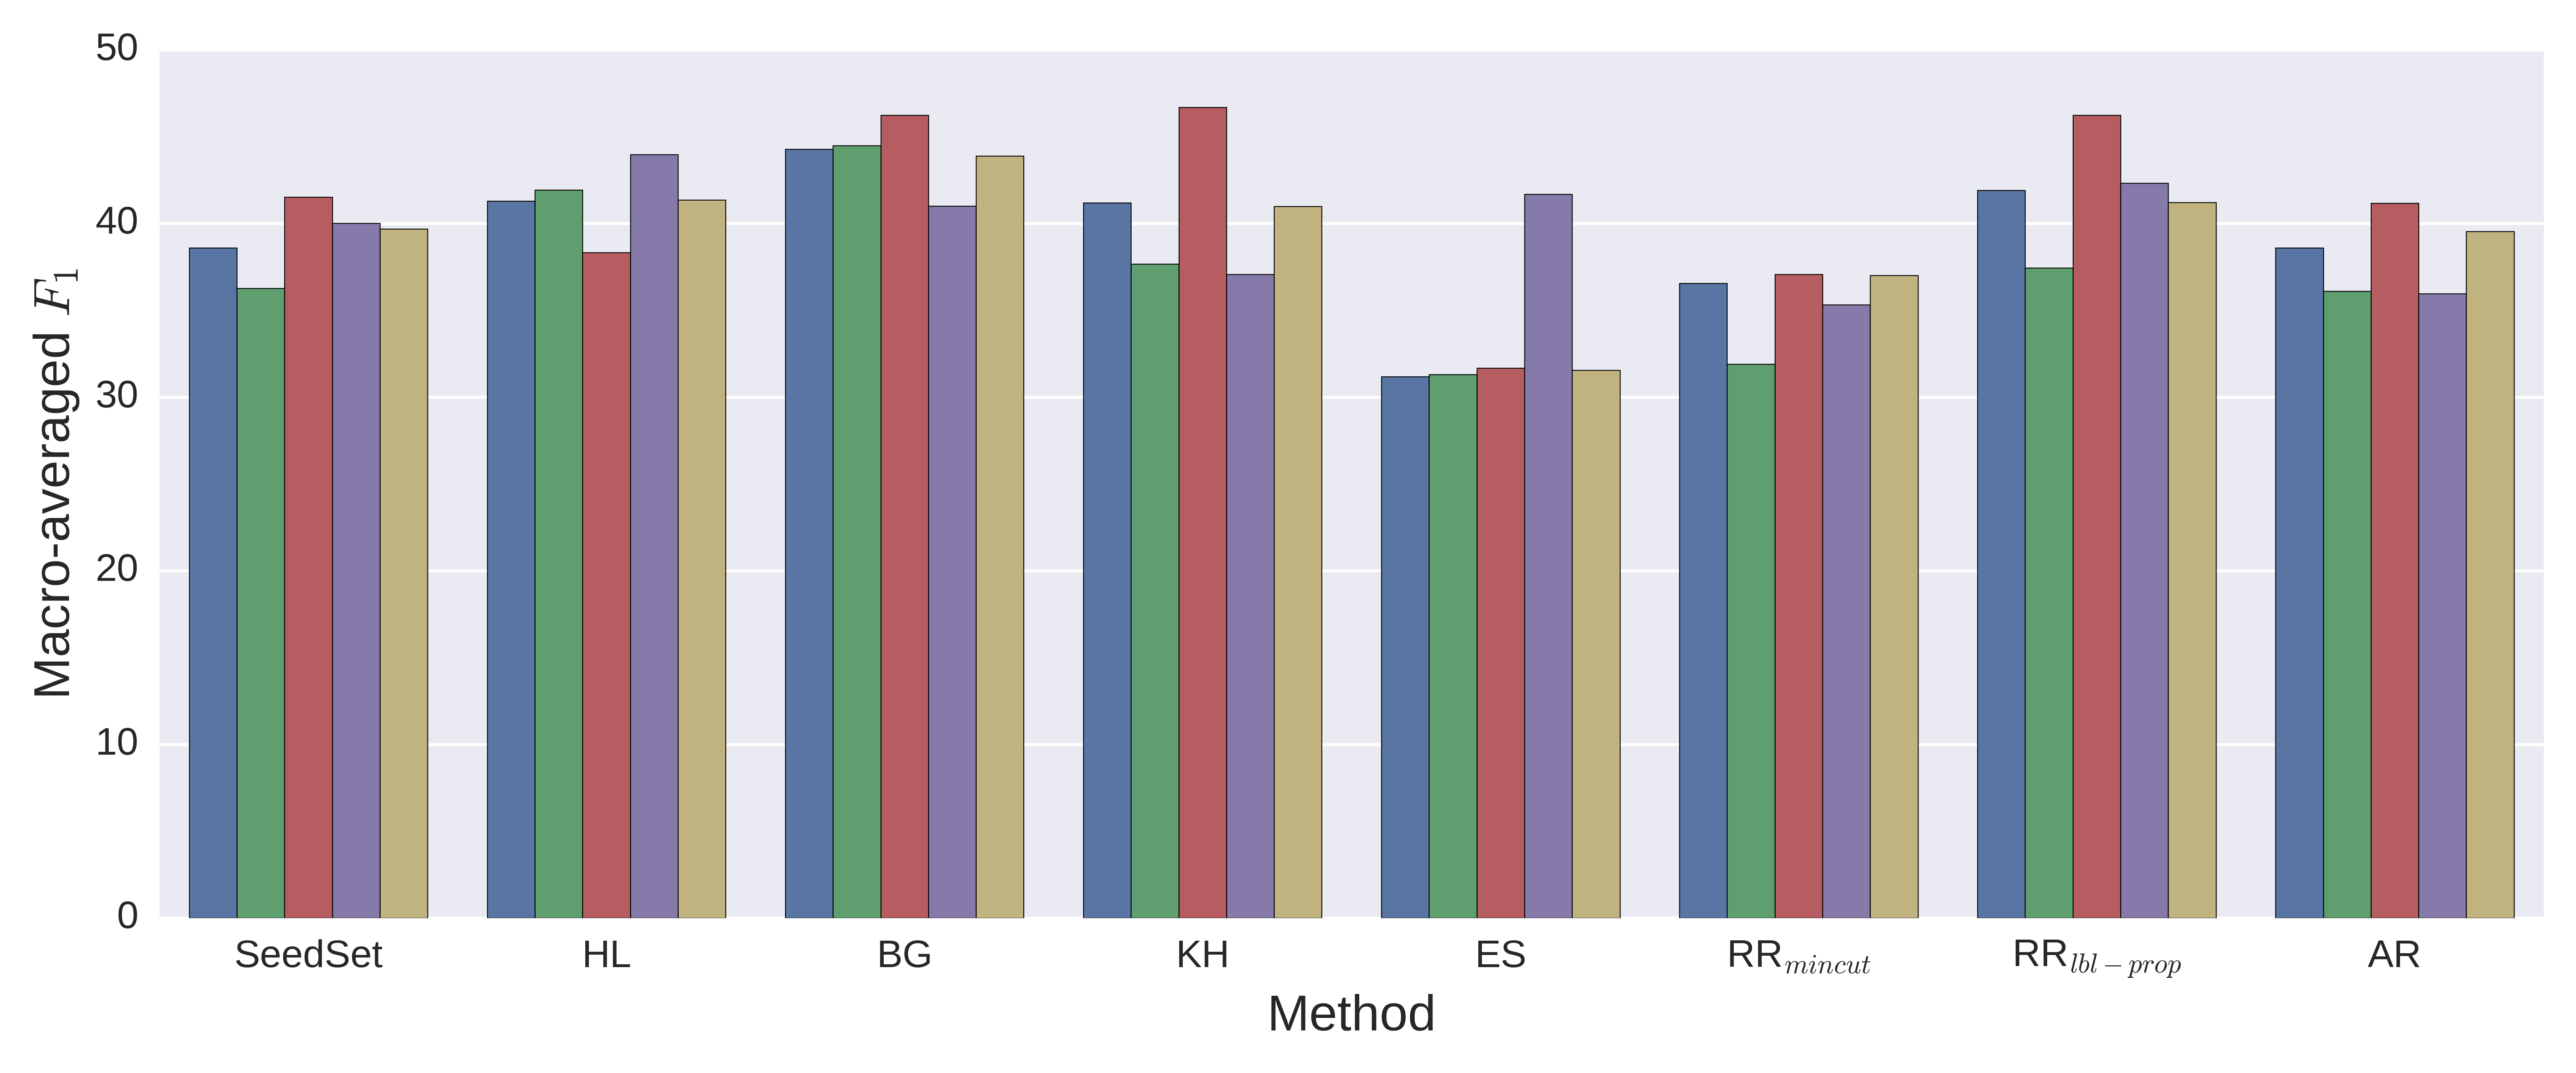
\includegraphics[width=\linewidth]{img/sentilex-alt-seed-sets.png}
}
\caption{Macro-averaged \F{}-scores of dictionary-based methods with
  different seed sets.\\ {\small (HL -- \citet{Hu:04}, BG --
    \citet{Blair-Goldensohn:08}, KH -- \citet{Kim:04,Kim:06}, ES --
    \citet{Esuli:06c}, RR -- \citet{Rao:09}, AR --
    \citet{Awadallah:10})}}\label{snt:fig:sent-lex-alt-seeds}
\end{figure}

For convenience, we will summarize the results of three top-performing
configurations---the methods of \citet{Blair-Goldensohn:08},
\citet{Kim:04,Kim:06}, and the label-propagation approach of
\citet{Rao:09} used in combination with the initial seed sed of
\citet{Kim:04}---in Table~\ref{snt-lex:tbl:lex-kh-seedset} and use
these results as baselines in our later experiments.

\begin{table}[h]
  \begin{center}
    \bgroup \setlength\tabcolsep{0.1\tabcolsep}\scriptsize
    \begin{tabular}{p{0.1\columnwidth} % first columm
        *{9}{>{\centering\arraybackslash}p{0.078\columnwidth}} % next nine columns
        *{2}{>{\centering\arraybackslash}p{0.078\columnwidth}}} % last two columns
      \toprule
          \multirow{2}*{\bfseries Lexicon} & %
          \multicolumn{3}{c}{\bfseries Positive Expressions} & %
          \multicolumn{3}{c}{\bfseries Negative Expressions} & %
          \multicolumn{3}{c}{\bfseries Neutral Terms} & %
          \multirow{2}{0.068\columnwidth}{\bfseries\centering Macro\newline \F{}} & %
          \multirow{2}{0.068\columnwidth}{\bfseries\centering Micro\newline \F{}}\\
          \cmidrule(lr){2-4}\cmidrule(lr){5-7}\cmidrule(lr){8-10}

          & Precision & Recall & \F{} & %
          Precision & Recall & \F{} & %
          Precision & Recall & \F{} & & \\\midrule

          BG & 22.7\stddev{6.5} & \textbf{29.9}\stddev{8.4} & 25.4\stddev{6.7} & %
          17.1\stddev{7.4} & \textbf{16.9}\stddev{7.2} & \textbf{16.6}\stddev{6.7} & %
          \textbf{97}\stddev{0.6} & 96.4\stddev{0.6} & 96.7\stddev{0.5} & %
          46.3\stddev{3.5} & 93.5\stddev{0.9}\\

          KH & 51.6\stddev{12.4} & 21.7\stddev{7.2} & \textbf{29.9}\stddev{8.1} & %
          38.9\stddev{24.7} & 7.5\stddev{4.9} & 12.2\stddev{7.8} & %
          96.7\stddev{0.7} & \textbf{99.4}\stddev{0.2} & \textbf{98}\stddev{0.4} & %
          \textbf{46.7}\stddev{3.9} & \textbf{96}\stddev{0.7}\\

          RR$_{\textrm{lbl-prop}}$ & \textbf{52.9}\stddev{15.2} & 18.4\stddev{6.5} & 26.7\stddev{8.2} & %
          \textbf{42.8}\stddev{29.7} & 8.9\stddev{5.8} & 14.1\stddev{8.8} & %
          96.6\stddev{0.7} & \textbf{99.4}\stddev{0.3} & \textbf{98}\stddev{0.4} & %
          46.3\stddev{4.3} & \textbf{96}\stddev{0.8}\\
          \bottomrule
    \end{tabular}
    \egroup
    \caption{Results of the top-scoring dictionary-based approaches
      with the best observed seed set configuration. {\small (BG --
        \citet{Blair-Goldensohn:08}, KH -- \citet{Kim:04,Kim:06}, RR
        -- \citet{Rao:09})}}
    \label{snt-lex:tbl:lex-kh-seedset}
  \end{center}
\end{table}

% Seed Sets:

% Hu-Liu were using 30 adjectives, but they only provided some
% examples: great, fantastic, nice, cool, bad, and dull

% Blair-Goldensohn: do not report (In our experiments, the original
% seed set contained 20 negative and 47 positive words that were
% selected by hand to maximize domain coverage, as well as 293 neutral
% words that largely consist of stop words.)

% Kim-Hovy (2004): To start the seed lists we selected verbs (23
% positive and 21 negative) and adjectives (15 positive and 19
% negative), adding nouns later.  But they, again, do not report
% specific examples.

% Kim-Hovy (2006): We described a word classification system to de-
% tect opinion-bearing words in Section 2.1. To ex- amine its
% effectiveness, we annotated 2011 verbs and 1860 adjectives, which
% served as a gold stan- dard 7 . These words were randomly selected
% from a collection of 8011 English verbs and 19748 English
% adjectives. We use training data as seed words for the WordNet
% expansion part of our algorithm.

% Esuli/Sebastiani: Lp and Ln are two small sets, which we have
% defined by manually selecting the intended synsets4 for 14
% "paradigmatic" Positive and Negative terms (e.g., the Positive term
% nice, the Negative term nasty) which were used as seed terms in
% (Turney and Littman, 2003).  The Lo set is treated differently from
% Lp and Ln, because of the inherently "complementary" nature of the
% Objective category (an Objective term can be defined as a term that
% does not have either Positive or Negative characteristics). We have
% heuristically defined Lo as the set of synsets that (a) do not
% belong to either T rK p or T rK n , and (b) contain terms not marked
% as either Positive or Negative in the General Inquirer lexicon
% (Stone et al., 1966); this lexicon was chosen since it is, to our
% knowledge, the largest manually annotated lexicon in which terms are
% tagged according to the Positive or Negative categories.

% Rao-Ravichandran: All experiments reported in Sections 4.1 to 4.5
% use the data described above with a 50-50 split so that the first half
% is used as seeds and the sec- ond half is used for test.

% Awdallah: After (Turney, 2002), we use our method to predict
% semantic orientation of words in the General Inquirer lexicon (Stone
% et al., 1966) using only 14 seed words.

% seed sets: (Turney and Littman, 2003); SentiWS (Remus, 2010)

\subsection{Evaluation of Corpus-Based Approaches}

An alternative way to generate polarity lists represent corpus-based
methods.  In contrast to dictionary-based approaches, these systems
typically do not require any large-scale hand-crafted linguistic
thesauri and draw their information directly from (untagged) corpus
data, harnessing the co-occurrence statistics of the initial seed
terms.  A clear advantage of such methods are their virtual
independence of any (expensive) language resources and the ability to
keep pace with frequent changes in the targeted discourse domain.
These benefits, however, come at the cost of a reduced quality as
these systems operate almost completely unsupervised.

A pioneering work on these methods was done by \citet{Hatzivassi:97}.
Based on the assumption that coordinatively connected adjectives
typically share the same semantic orientation, the authors trained a
supervised logisitic regression classifier, which predicted the degree
of dissimilarity between two conjoined adjectival terms.  In the next
step, they constructed a word graph, drawing a link between any two
adjectives if they appeared in the same coordination pair and taking
the predicted dissimilarity scores as edge weights in the constructed
graph.  In the final step, \citet{Hatzivassi:97} partitioned the final
graph into two parts and ascribed positive polarity to the cluster
which had more nodes.  This method achieved an overall accuracy of
82.05\% on predicting the polarity of a subset of manually annotated
adjectives when trained on the rest of these hand-labeled data.

Later on, this approach was further refined by \citet{Takamura:05},
who tried to unite dictionary- and corpus-based methods into a unified
probabilistic framework.  To this end, the authors adopted the Ising
spin model from the statistical mechanics, considering terms from
\textsc{WordNet} \cite{Miller:95}, the Wall Street Journal and Brown
corpora as electrons in a single ferromagnetic lattice.  A link was
established between any two electrons, if their corresponding terms
appeared in synonymically connected synsets or a coordinatively
conjoined pair in any of the two corpora.  Taking into account the a
priori known polarities of the seed terms, the Ising model then tried
to find an approximation of the most likely polarity combination of
all terms in the graph over all possible polarity assignments,
reaching 91.5\% accuracy at predicting polarity of the manually
labeled subjective terms from the General Inquirer lexicon
\cite{Stone:66}.

An alternative way of inducing sentiment lexicons was proposed by
\citet{Turney:03}, who derived a set of polarity terms by computing
the ratio of PMI-associations between the potential items and
predefined sets of positive and negative seeds.  In particular, the
semantic orientation score of the given word $w$ was defined as:
\begin{equation*}
  \textrm{SO-A}(w) = \sum_{w_p\in\mathcal{P}}PMI(w, w_p) - \sum_{w_n\in\mathcal{N}}PMI(w, w_n),
\end{equation*}
where $\mathcal{P}$ was the set of the positive seed terms (presented
earlier in this sections), $\mathcal{N}$ denoted the collection of the
negative words, and the $PMI$ score was normally computed as the
log-ratio $PMI(w, w_x) = \log_2\frac{p(w, w_x)}{p(w)p(w_x)}$.  The
joint probability $p(w, w_x)$ was calculated with the help of the
AltaVista\footnote{\url{www.altavista.com}} NEAR operator as the
number of hits returned by the $w NEAR w_x$ query divided by the total
number of indexed documents.

With great success, this method was later adapted to the Twitter
domain by \citet{Kiritchenko:14}.  Using the distantly supervised
corpus of \citet{Go:09} and a separate collection of 775,000 tweets
gathered solely for the purpose of their experiments, the authors
created two sentiment lexicons---the Sentiment140 Base Lexicon and
Hashtag Sentiment Base Lexicon respectively---using the semantic
orientation formula described above.  However, instead of querying
AltaVista for computing the joint probability scores, the authors
estimated these values as the number of times a potential candidate
appeared in a positive (negative) tweet divided by the total number of
tweets in the collection.  The polarity classes of the tweets were
distantly assigned based on the occurrence of predefined emoticons in
the \citet{Go:09} corpus or emotional hashtags in the compiled tweet
collection.

Later on, this approach was further refined by \citet{Severyn:15a},
who compiled their list of polar terms by training an SVM classifier
on the distantly suervised corpus of \citet{Go:09}, using solely
lexical n-gram features.  In the final step, features with the highest
learned weights were selected as subjective entries for the
constructed sentiment lexicon.

Graphical methods for corpus-based lexicon induction were advocated by
\citet{Velikovich:10} and \citet{Feng:11}.  The former work proposed
an adaptation of the label-propagation algorithm previously suggested
by \citet{Rao:09} with the core difference that, instead of taking a
weightes average of all incident scores for a potential subjective
term, the authors took the maximum value propagated from a seed to the
potential candidate over the lexical graph.  \citet{Feng:11}
experimented with two popular IR approaches---PageRank \cite{Brin:98}
and HITS \cite{Kleinberg:99}---to derive lists of predicates
typically associated with positively or negatively connotated events
and these events themselves.

\cite{Lau:11}

\citet{Bross:13}

\citet{Tai:13}

\citet{Yang:14}

\citet{Bravo-Marquez:15}

\begin{figure}[hbtp!]
{
  \centering
  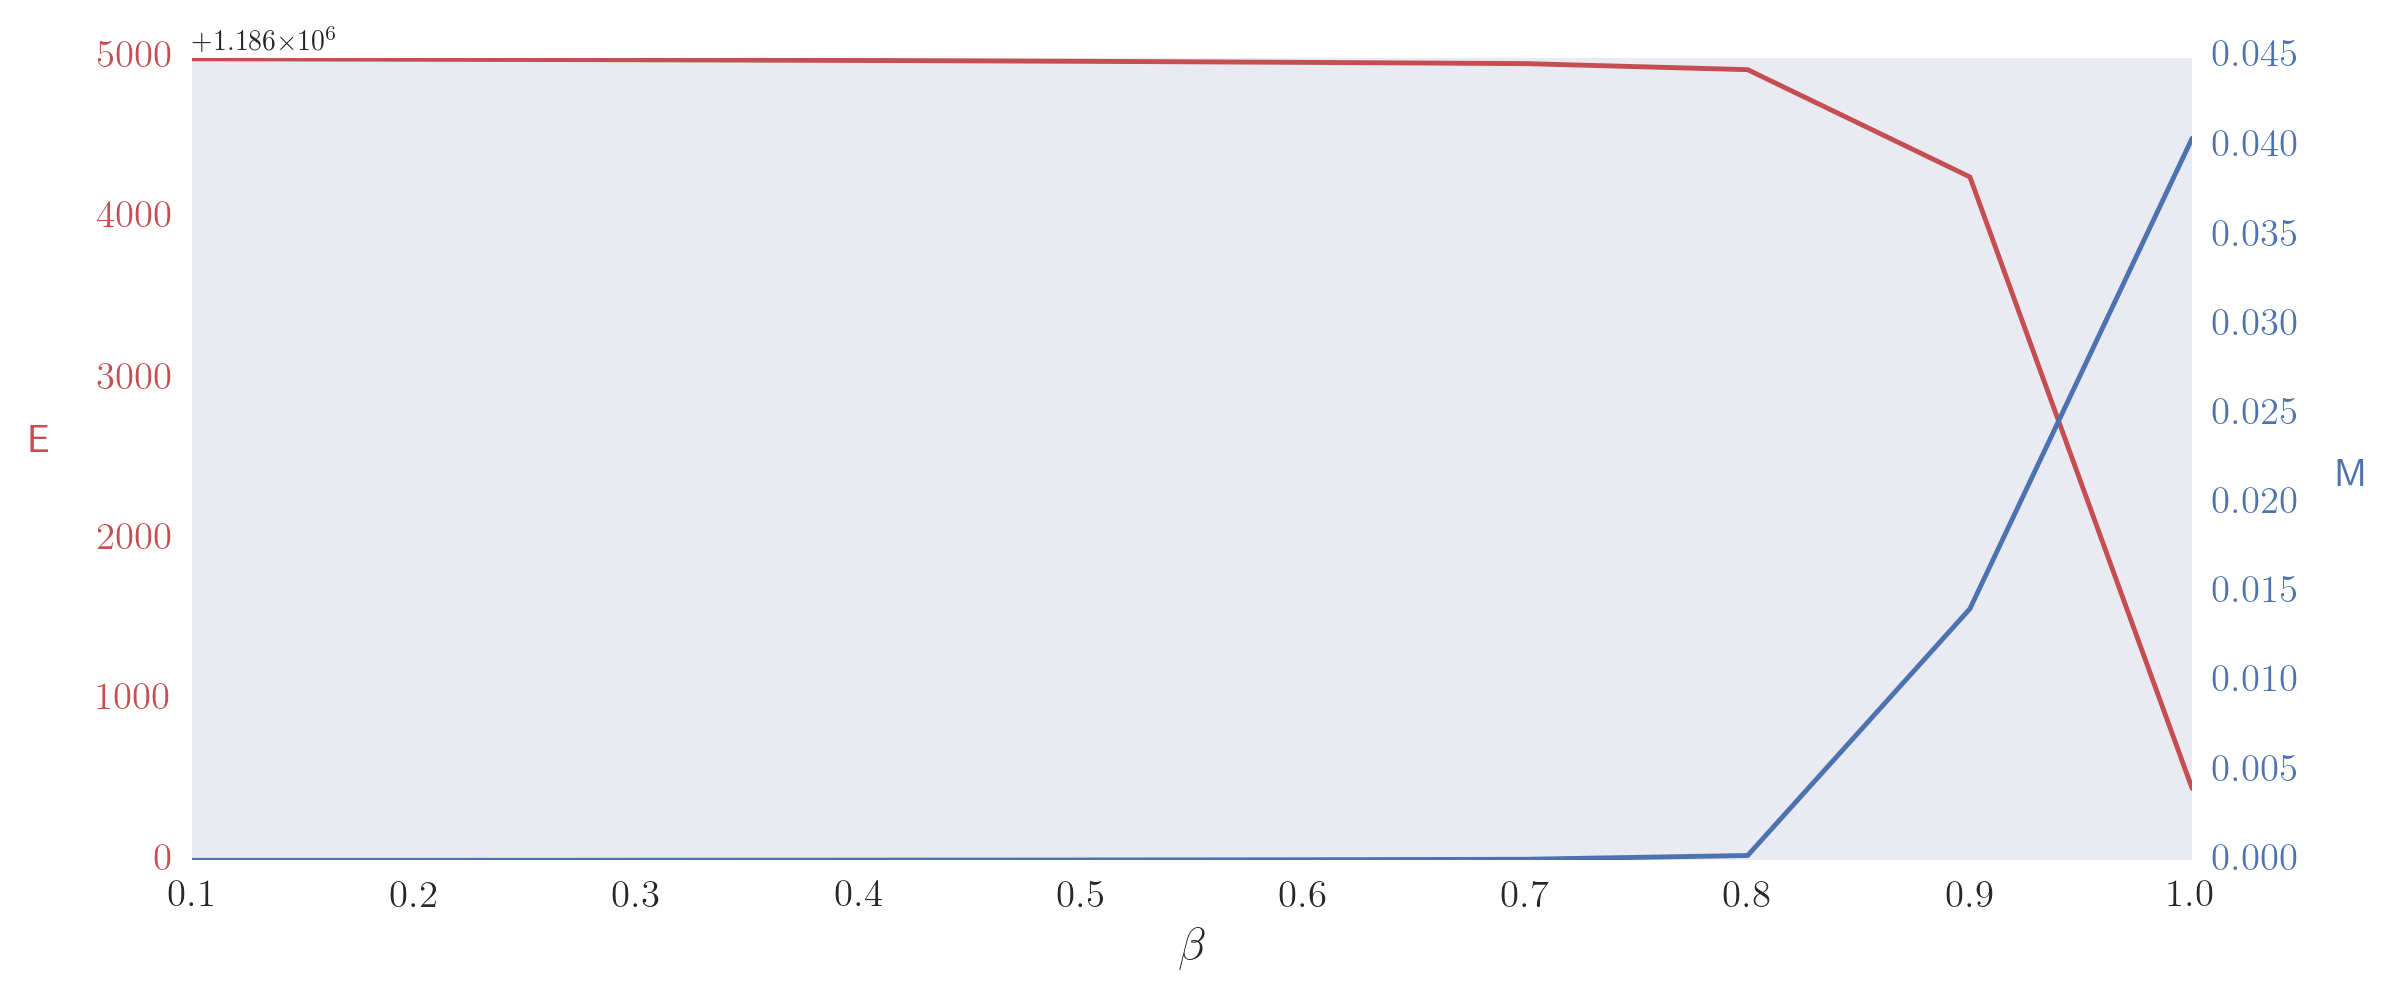
\includegraphics[width=\linewidth]{img/ising-energy-magnetization.png}
}
\caption{Energy (E) and magnetization (M) if the Ising spin model with
  respect to the hyper-parameter $\beta$.}\label{snt:fig:ising-spin-em}
\end{figure}

In order to see which of the two paradigms---dictionary-based methods
or corpus-based approaches---bears more potential for generating
high-quality sentiment lexicons for Twitter, we re-implemented the
most popular systems from the latter group and evaluated these methods
on our corpus.  The results of these computations are presented in
Table~\ref{snt-lex:tbl:corp-meth}.

\begin{table}[h]
  \begin{center}
    \bgroup \setlength\tabcolsep{0.1\tabcolsep}\scriptsize
    \begin{tabular}{p{0.1\columnwidth} % first columm
        *{9}{>{\centering\arraybackslash}p{0.078\columnwidth}} % next nine columns
        *{2}{>{\centering\arraybackslash}p{0.078\columnwidth}}} % last two columns
      \toprule
          \multirow{2}*{\bfseries Lexicon} & %
          \multicolumn{3}{c}{\bfseries Positive Expressions} & %
          \multicolumn{3}{c}{\bfseries Negative Expressions} & %
          \multicolumn{3}{c}{\bfseries Neutral Terms} & %
          \multirow{2}{0.068\columnwidth}{\bfseries\centering Macro\newline \F{}} & %
          \multirow{2}{0.068\columnwidth}{\bfseries\centering Micro\newline \F{}}\\
          \cmidrule(lr){2-4}\cmidrule(lr){5-7}\cmidrule(lr){8-10}

          & Precision & Recall & \F{} & %
          Precision & Recall & \F{} & %
          Precision & Recall & \F{} & & \\\midrule

          % cardinality 2,560; \beta = 0.1
          TKM & 48.8\stddev{17.9} & 12.4\stddev{5.9} & 19.3\stddev{7.9} & %
          35.7\stddev{28.7} & 4.5\stddev{3.9} & 7.7\stddev{6.4} & %
          96.4\stddev{0.8} & 99.6\stddev{0.2} & 98\stddev{0.4} & %
          41.7\stddev{3.7} & 96\stddev{0.8}\\

          VEL & \stddev{} & \stddev{} & \stddev{} & %
          \stddev{} & \stddev{} & \stddev{} & %
          \stddev{} & \stddev{} & \stddev{} & %
          \stddev{} & \stddev{}\\

          KIR & \stddev{} & \stddev{} & \stddev{} & %
          \stddev{} & \stddev{} & \stddev{} & %
          \stddev{} & \stddev{} & \stddev{} & %
          \stddev{} & \stddev{}\\

          SM & \stddev{} & \stddev{} & \stddev{} & %
          \stddev{} & \stddev{} & \stddev{} & %
          \stddev{} & \stddev{} & \stddev{} & %
          \stddev{} & \stddev{}\\
          \bottomrule
    \end{tabular}
    \egroup
    \caption{Evaluation of corpus-based approaches.\\ {\small (TKM --
        \citet{Takamura:05}), VEL -- \citet{Velikovich:10}, KIR --
        \citet{Kiritchenko:14}, SM -- \citet{Severyn:15a}}}
    \label{snt-lex:tbl:corp-meth}
  \end{center}
\end{table}

\subsection{Lexicon Generation Using Neural Word Embeddings}

\citet{Tang:14}

\citet{Tang:14a}

Similarly to \citet{Severyn:15a}, \citet{Vo:16} applied a deep
learning approach learning two-dimensional embeddings (one dimension
for the positive score and one dimension for the negative appraisal)

\citet{Ren:16}

A new family of lexicon induction methods builds on learned vector
representations of words -- the neural word embeddings
\cite{Mikolov:13}.

Vector command:
\begin{verbatim}
Adjusted Potts' Tokenizer

Sidarenka's Preprocessing (Smiley Replacement)

word2vec -train tokens.tok -output vectors.txt -size 400 -window 5 -min-count 4

Possible Improvements:

* use task specific vectors;

* decide what to do with smileys during evaluation;

* explore different cardinalities (not just 40-s bins);
\end{verbatim}

% k-NN: k^2 / \sum d_{ij}

The results of these methods are shown in Table~\ref{snt-lex:tbl:nwe-methods}.

\begin{table}[h]
  \begin{center}
    \bgroup \setlength\tabcolsep{0.1\tabcolsep}\scriptsize
    \begin{tabular}{p{0.1\columnwidth} % first columm
        *{9}{>{\centering\arraybackslash}p{0.078\columnwidth}} % next nine columns
        *{2}{>{\centering\arraybackslash}p{0.078\columnwidth}}} % last two columns
      \toprule
          \multirow{2}*{\bfseries Lexicon} & %
          \multicolumn{3}{c}{\bfseries Positive Expressions} & %
          \multicolumn{3}{c}{\bfseries Negative Expressions} & %
          \multicolumn{3}{c}{\bfseries Neutral Terms} & %
          \multirow{2}{0.068\columnwidth}{\bfseries\centering Macro\newline \F{}} & %
          \multirow{2}{0.068\columnwidth}{\bfseries\centering Micro\newline \F{}}\\
          \cmidrule(lr){2-4}\cmidrule(lr){5-7}\cmidrule(lr){8-10}

          & Precision & Recall & \F{} & %
          Precision & Recall & \F{} & %
          Precision & Recall & \F{} & & \\\midrule

          % cardinality 160
          NC & 75.7\stddev{23.8} & 9.1\stddev{5.7} & 15.8\stddev{8.8} & %
          24.4\stddev{41.8} & 1\stddev{1.8} & 1.9\stddev{3.4} & %
          96.3\stddev{0.8} & \textbf{99.9}\stddev{0.1} & \textbf{98.1}\stddev{0.4} & %
          38.6\stddev{3.2} & \textbf{96.2}\stddev{0.8}\\

          % cardinality 40
          KNN & \textbf{75.8}\stddev{23.8} & 9.1\stddev{5.7} & 15.8\stddev{8.8} & %
          23.4\stddev{40.6} & 1\stddev{1.8} & 1.8\stddev{3.4} & %
          96.3\stddev{0.8} & \textbf{99.9}\stddev{0.1} & \textbf{98.1}\stddev{0.4} & %
          38.6\stddev{3.2} & \textbf{96.2}\stddev{0.8}\\

          % cardinality 160
          PCA & 40.4\stddev{14.6} & \textbf{13.4}\stddev{5.8} & \textbf{19.5}\stddev{7.3} & %
          24.4\stddev{41.8} & 1\stddev{1.8} & 1.9\stddev{3.4} & %
          \textbf{96.4}\stddev{0.8} & 99.6\stddev{0.2} & 97.9\stddev{0.4} & %
          39.8\stddev{2.7} & 95.9\stddev{0.8}\\

          % cardinality 160
          LP & \textbf{75.8}\stddev{23.8} & 9.1\stddev{5.7} & 15.8\stddev{8.8} & %
          \textbf{29.4}\stddev{20.3} & \textbf{5.6}\stddev{4.5} & \textbf{9.2}\stddev{6.9} & %
          \textbf{96.4}\stddev{0.8} & 99.8\stddev{0.1} & 98\stddev{0.4} & %
          \textbf{41}\stddev{3.9} & 96.1\stddev{0.8}\\
          \bottomrule
    \end{tabular}
    \egroup
    \caption{Evaluation of embedding-based approaches.\\ {\small (NC
        -- nearest centroids, KNN -- k-nearest neighbors, PCA --
        principal component analysis, LP -- linear projection)}}
    \label{snt-lex:tbl:nwe-methods}
  \end{center}
\end{table}

\subsection{Discussion}

Since \textsc{GermaNet}, however, is significantly different from its
English counterpart, both quantitatively and qualitatively, we should
first present some key statistics (shown in
Table~\ref{snt-lex:tbl:germanet-wordnet}) and visualize the synset
graphs (demonstrated in Figures~\ref{snt-lex:fig:germanet}
and~\ref{snt-lex:fig:wordnet}) of these lexical databases.

\begin{table}[h]
  \begin{center}
    \bgroup \setlength\tabcolsep{0.1\tabcolsep}\scriptsize \small
    \begin{tabular}{p{0.15\textwidth} % first columm
        *{8}{>{\centering\arraybackslash}m{0.085\textwidth}}} % next nine columns
      \toprule
      & \multicolumn{2}{c}{\bfseries Noun} & %
      \multicolumn{2}{c}{\bfseries Verb} & %
      \multicolumn{2}{c}{\bfseries Adjective} & & \\
      \multirow{-2}{0.12\columnwidth}{\centering\bfseries Resource} & %
      Words & Synsets & Words & Synsets & Words & Synsets & %
      \multirow{-2}{0.085\columnwidth}{\centering\scriptsize\bfseries{}Hy\-pon.\newline{}Rels} & %
      \multirow{-2}{0.085\columnwidth}{\centering\scriptsize\bfseries{}Anto\-n.\newline{}Rels}\\
      \midrule

      \textsc{GermaNet} & 85,662 & 71,575 & 9,340 & 11,026 & 12,890 & 10,645 & %
      97,712 & 1,741\\
      \textsc{WordNet}  & 117,798 & 82,115 & 11,529 & 13,767 & 21,479 & 18,156 & %
      95,322 & 7,394\\
      \bottomrule
    \end{tabular}
    \egroup
    \caption{Key statistics on \textsc{GermaNet} and
      \textsc{WordNet}.}
    \label{snt-lex:tbl:germanet-wordnet}
  \end{center}
\end{table}

\begin{figure*}[htbp!]
{
\centering
\begin{subfigure}{.5\textwidth}
  \centering
  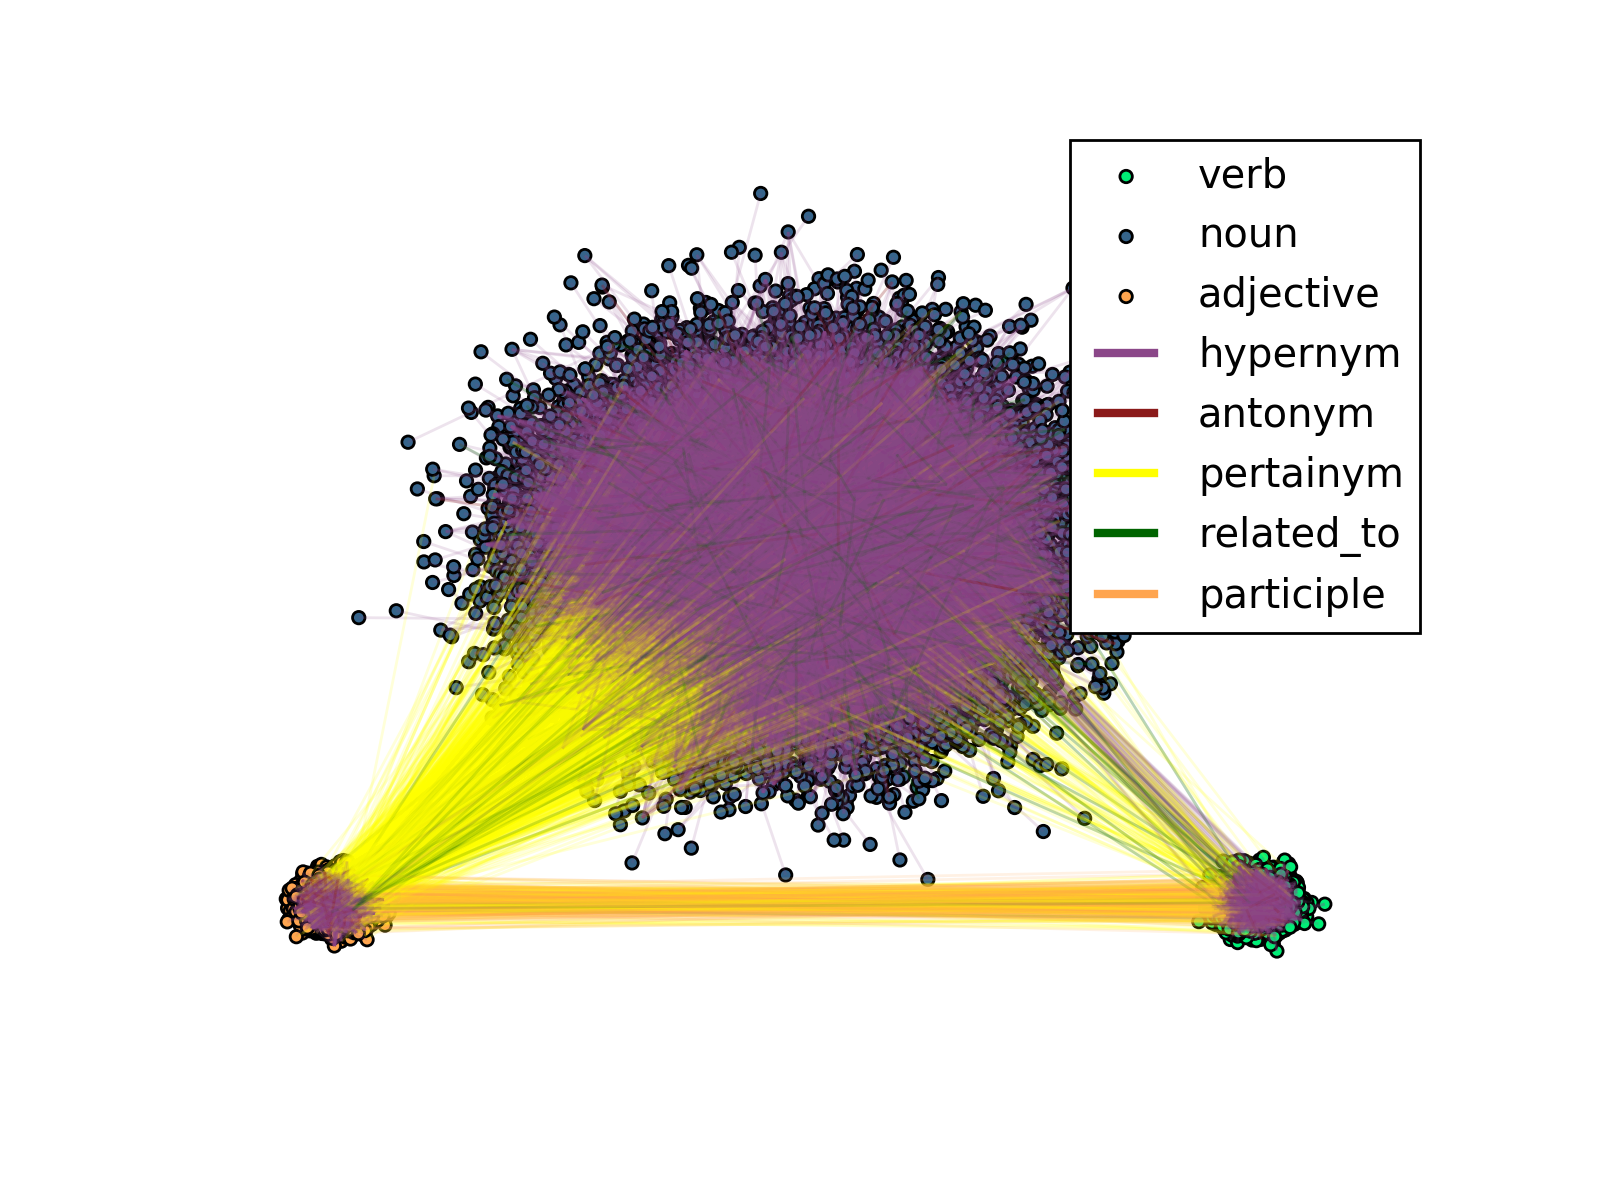
\includegraphics[width=\linewidth]{img/germanet.png}
  \caption{\textsc{GermaNet}}\label{snt-lex:fig:germanet}
\end{subfigure}%
\begin{subfigure}{.5\textwidth}
  \centering
  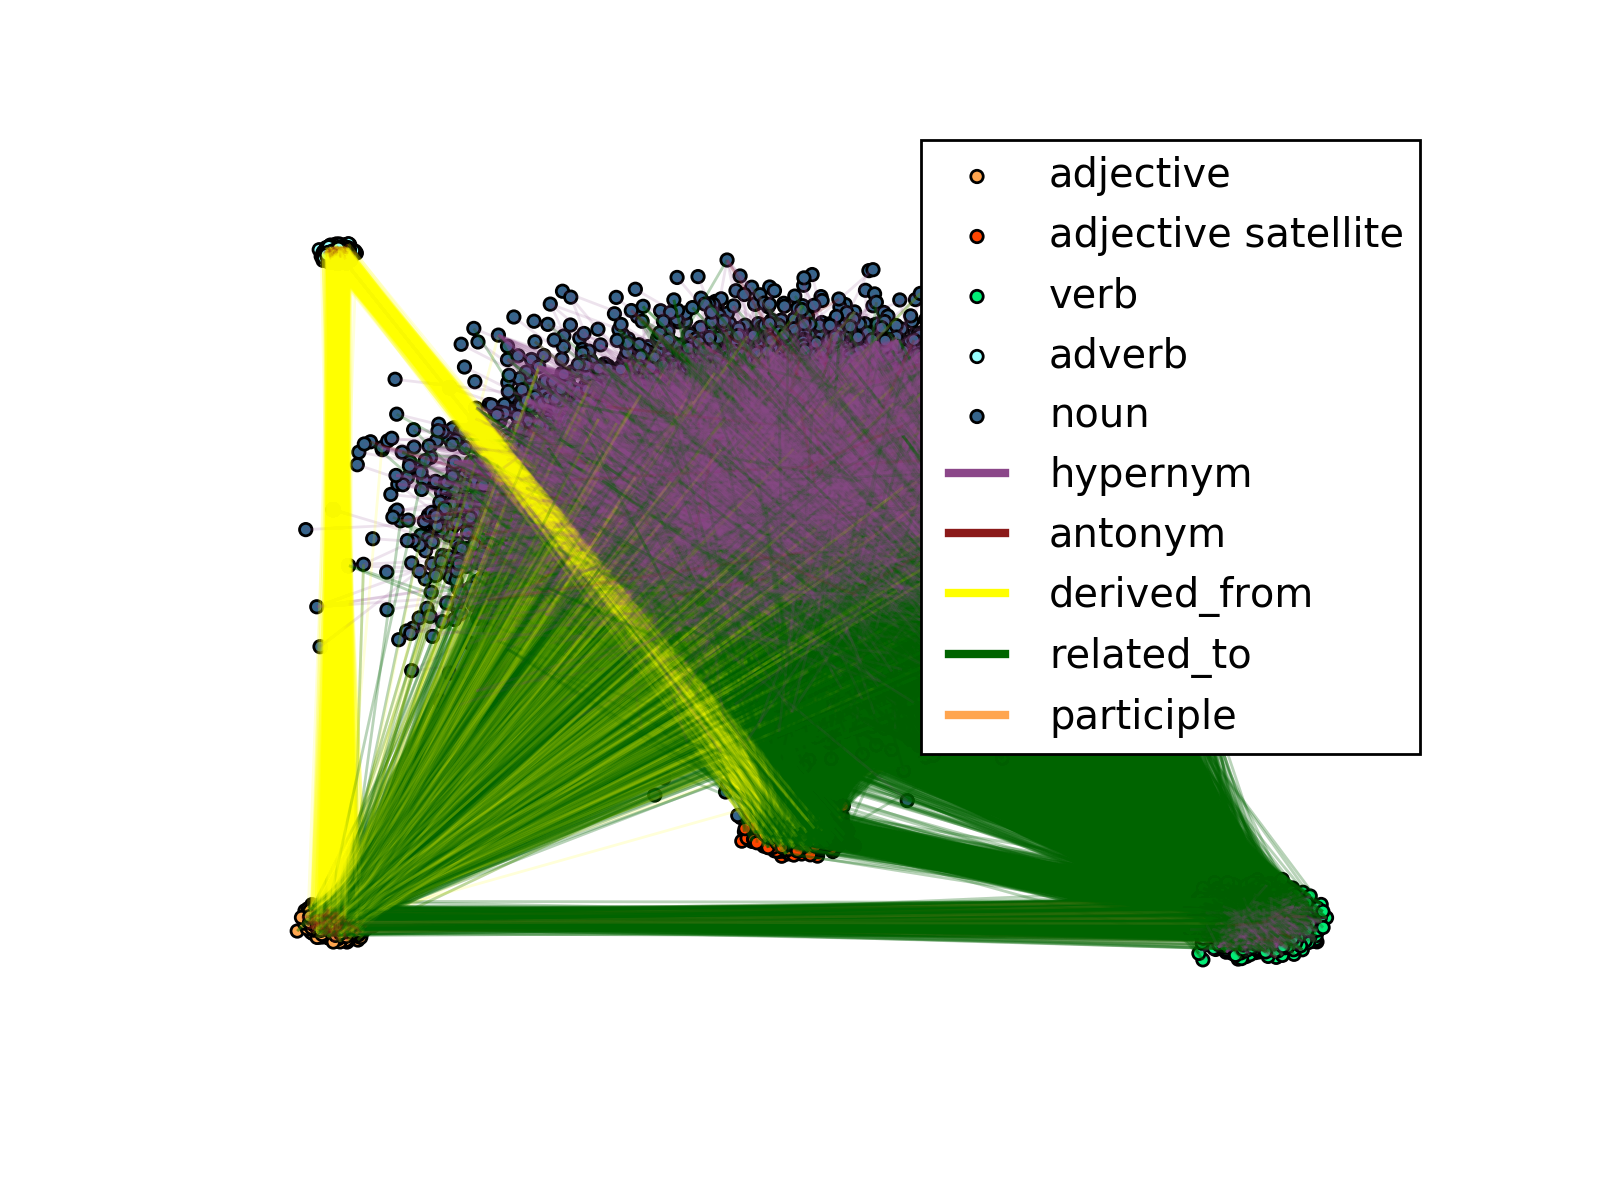
\includegraphics[width=\linewidth]{img/wordnet.png}
  \caption{\textsc{WordNet}}\label{snt-lex:fig:wordnet}
\end{subfigure}
}
\caption{Graphical visualization of \textsc{GermaNet} and
      \textsc{WordNet}.}\label{snt:fig:crp-sent-emo-distr}
\end{figure*}

As can be seen from the table, \textsc{GermaNet} has significantly
fewer words and synsets for all common parts of speech with the
largest gaps observed for nouns and adjectives.  Moreover, as shown in
Figures~\ref{snt-lex:fig:germanet} and~\ref{snt-lex:fig:wordnet}, such
PoS-classes as adverbs and adjective satellites are completely missing
in the German resource.  The reason for this is that the form (and
meaning) of most German adverbs typically coincides with that of the
adjectives; therefore, both categories are treated in the same way,
being represented through the adjectival synsets.

A slightly different situation can be observed for the semantic links
(relations) between the synsets: here, \textsc{GermaNet} features
almost 2,500 more hypernym-hyponym pairs than the English resource,
whereas the number of antonyms is more than four times less than in
\textsc{WordNet}.

An especially interesting pattern, however, appears with the relations
connecting different parts of speech: As can be seen from the figures,
the strongest inter-PoS connections in \textsc{GermaNet} are the
pertainym links between the adjectives and nouns and the participle
edges between the adjectives and verbs.  The interlinks between the
nouns and verbs, however, are both much fewer in number and more
diverse in their nature.  This situation is different in
\textsc{WordNet} where the prevailing majority of the
inter-part-of-speech connections are represented through the
\texttt{related\_to} (especially between the nouns, adjective
satellites, verbs, and verbs and adjectives) and
\texttt{derived\_from} links (especially between adverbs and
adjectives with their satellites).  The relations between the
adjectives and nouns are mixed though, featuring both
\texttt{related\_to} and \texttt{derived\_from} connections.  As we
should see later, these links are crucial for breaking part-of-speech
dependencies of seed sets in the cases when all seeds belong to the
same PoS class.

Another lexical sentiment resource (\textsc{WordNet-Affect}) was
proposed by \citet{Strapparava:04} who manually compiled a list of
1,903 subjective terms and projected these polarities to the
respective synononyms set in \textsc{WordNet}.  The resulting database
included 2,874 synsets with a total of 4,787 words.

% \subsubsection{Domain-Specific Sentiment Lexica}

% \citet{Chetviorkin:14} obtained a set of possible subjective terms
% from English and Russian microblogs by using an ensemble of supervised
% machine learning classifiers that had previously been trained on a
% manually annotated corpus of movie reviews.  In order to determine the
% prior polarity of the extracted terms, the authors first calculated
% approximate polarity scores of the processed messages using general
% polarity lexicons and then took these rough estimates as prior
% polarity expectations of the candidate expressions.  The posterior
% scores of these expressions were computed using the Ising spin model
% in a similar way to the approach proposed by \citet{Takamura:05}.  The
% resulting lexicon comprised 2,772 words for Russian and 2,786 lexical
% items for English.

\subsection{Summary and Conclusions}

In this section, we presented the first attempt of a practical
evaluation of our corpus.  In doing so, we addressed the task of
automatic prediction of polar terms (emotional expressions) with the
help of sentiment dictionaries.  To obtain a rough baseline estimate,
we first evaluated the quality of the existing sentiment lists for
German: German Polarity Clues~\cite{Waltinger:10},
SentiWS~\cite{Remus:10}, and Zurich Polarity List~\cite{Clematide:10}.
We showed that \ldots achieved the best quality, reaching an average
\F{}-score of \ldots on recognizing positive expressions and \ldots on
predicting negative polar terms.

In the next step, we analyzed whether the methods that were used for
creating the original English resources whose translations formed the
basis of the German lexica could yield better results than the
manually revised tranlated lists when applied to German data directly.

Another popular approach to an unsupervised induction of sentiment
lexica relies on the cooccurrence information about the words taken
directly from corpus.  One of the most popular methods from this
category is the Ising spin model adopted from the statistical
mechanics which interprets words as magnetic spins in a crystal grid
and tries to derive the most probable orientation of these spins in a
magnetic field.  This model was first applied to the needs of
computational linguistics by \citet{Takamura:05}, who induced a
sentiment lexicon for English using \ldots corpus data.  We have
reimplemented this approach in our program suite and applied to the
German Twitter snapshop of \citet{Scheffler:14}.  The results of this
approach are shown in Table~\ref{snt-lex:tbl:ispn-res}.

A different way of incorporating corpus data is to encode the
cooccurrence statistics directly into word information, representing
the latter as vectors.  We explored this direction in the final part
of this section, first obtaining word2vec embeddings for tokens from
the aforementioned snapshot and then applying clustering algorithms to
these representations.

Our results show that \ldots.

\newpage
